\documentclass[12pt]{article}

\usepackage[english]{babel}
\usepackage[UKenglish] {isodate}
\usepackage{amssymb, amsmath, calligra, mathrsfs, mathtools, color, enumitem, amsthm, hyperref, graphicx, array, tikz-cd, subfiles, footnote, titling, lipsum}
\usepackage[a4paper, top=2.2cm, bottom=2.5cm, left=1.8cm, right=1.8cm]{geometry}

\usepackage[all]{xy}
\usetikzlibrary{arrows}
\newtheorem{theorem}{Theorem}[section]
\newtheorem{lemma}[theorem]{Lemma}
\newtheorem{proposition}[theorem]{Proposition}
\newtheorem{corollary}[theorem]{Corollary}
\newtheorem{conjecture}[theorem]{Conjecture}
\newtheorem*{conjecture*}{Conjecture}
\theoremstyle{definition}
\newtheorem{definition}[theorem]{Definition}
\newtheorem{remark}[theorem]{Remark}
\newtheorem{fact}[theorem]{Fact}
\newtheorem{example}[theorem]{Example}
\newtheorem{algorithm}[theorem]{Algorithm}
\newtheorem{notation}[theorem]{Notation}
\newtheorem{setup}[theorem]{Set-up}
\newtheorem*{question*}{Question}
\numberwithin{equation}{subsection}
\renewcommand{\O}{\mathcal{O}}
\newcommand{\degree}{\ensuremath{^\circ}}
\newcommand{\coffe}{co\"effici\"ent }
\newcommand{\coffeen}{co\"effici\"enten }
\newcommand{\commentaar}[1]{}
\newcommand{\C}{\ensuremath{\mathbb{C}}}
\newcommand{\R}{\ensuremath{\mathbb{R}}}
\newcommand{\Q}{\ensuremath{\mathbb{Q}}}
\newcommand{\Z}{\ensuremath{\mathbb{Z}}}
\newcommand{\N}{\ensuremath{\mathbb{N}}}
\newcommand{\F}{\ensuremath{\mathbb{F}}}
\newcommand{\A}{\ensuremath{\mathbb{A}}}
\renewcommand{\P}{\ensuremath{\mathbb{P}}}
\newcommand{\GL}{\ensuremath{\mathrm{GL}}}
\newcommand{\T}{\textrm{T}}
\newcommand{\Hom}{\textrm{Hom}}
\DeclareMathOperator{\ShHom}{\mathscr{H}\text{\kern -3pt {\calligra\large om}}\,}
\renewcommand{\O}{\mathcal{O}}
\newcommand{\vol}{\mathop{\mathrm{vol}}}
\renewcommand{\Re}{\mathop{\mathrm{Re}}}
\renewcommand{\Im}{\mathop{\mathrm{Im}}}
\newcommand{\Div}{\mathrm{Div}}
\newcommand{\PDiv}{\mathrm{PDiv}}
\newcommand{\Pic}{\mathrm{Pic}}
\newcommand{\p}{\mathfrak{p}}
\renewcommand{\div}{\mathop\mathrm{div}}
\newcommand{\Proj}{\mathop\mathrm{Proj}}
\newcommand{\Spec}{\mathop\mathrm{Spec}}
\newcommand{\Spf}{\mathop\mathrm{Spf}}
\newcommand{\Specmax}{\mathop\mathrm{Specmax}}
\newcommand{\Sch}{\mathbf{Sch}}
\newcommand{\op}{\ensuremath{^{\textrm{op}}}}
\newcommand{\Ab}{\mathbf{Ab}}
\newcommand{\Lie}{\mathrm{Lie}}
\newcommand{\stacks}[1]{\textrm{\cite[\href{http://stacks.math.columbia.edu/tag/#1}{#1}]{stacks}}}
\newcommand{\et}{\textrm{\'et}}
\newcommand{\tors}{\mathrm{tors}}
\newcommand{\rkan}{\mathrm{rk}_{\mathrm{an}}}
\makesavenoteenv{tabular}
\setlength{\parindent}{0pt}
\setlength{\parskip}{0.5\baselineskip}
\relpenalty=10000
\binoppenalty=10000
\setlength{\parindent}{0pt}

\DeclareFontFamily{U}{wncy}{}
\DeclareFontShape{U}{wncy}{m}{n}{<->wncyr10}{}
\DeclareSymbolFont{mcy}{U}{wncy}{m}{n}
\DeclareMathSymbol{\Sh}{\mathord}{mcy}{"58} 

\newcommand{\onlyinsubfile}[1]{#1}

\let\MakeUppercase\small

\newcommand{\latteen}{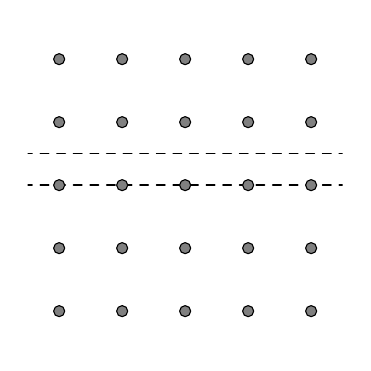
\begin{tikzpicture}[line cap=round,line join=round,>=triangle 45,x=0.8cm,y=0.8cm]\clip(-0.5,-0.5) rectangle (4.5,4.5);\draw [line width=0.6pt,domain=-1.8801411349281567:5.73722094225949,dashed] plot(\x,{(--8-0*\x)/4});\draw [line width=0.6pt,domain=-1.8801411349281567:5.73722094225949,dashed] plot(\x,{2.5});
\begin{scriptsize}\draw [fill=gray] (0,0) circle(2.0pt);\draw [fill=gray] (1,0) circle(2.0pt);\draw [fill=gray] (2,0) circle(2.0pt);\draw [fill=gray] (3,0) circle(2.0pt);\draw [fill=gray] (4,0) circle(2.0pt);\draw [fill=gray] (4,1) circle(2.0pt);\draw [fill=gray] (3,1) circle(2.0pt);\draw [fill=gray] (2,1) circle(2.0pt);\draw [fill=gray] (1,1) circle(2.0pt);\draw [fill=gray] (0,1) circle(2.0pt);\draw [fill=gray] (0,2) circle(2.0pt);\draw [fill=gray] (1,2) circle(2.0pt);\draw [fill=gray] (2,2) circle(2.0pt);\draw [fill=gray] (3,2) circle(2.0pt);\draw [fill=gray] (4,2) circle(2.0pt);\draw [fill=gray] (4,3) circle(2.0pt);\draw [fill=gray] (3,3) circle(2.0pt);\draw [fill=gray] (2,3) circle(2.0pt);\draw [fill=gray] (1,3) circle(2.0pt);\draw [fill=gray] (0,3) circle(2.0pt);\draw [fill=gray] (0,4) circle(2.0pt);\draw [fill=gray] (1,4) circle(2.0pt);\draw [fill=gray] (2,4) circle(2.0pt);\draw [fill=gray] (3,4) circle(2.0pt);\draw [fill=gray] (4,4) circle(2.0pt);\end{scriptsize}\end{tikzpicture}}

\newcommand{\latttwee}{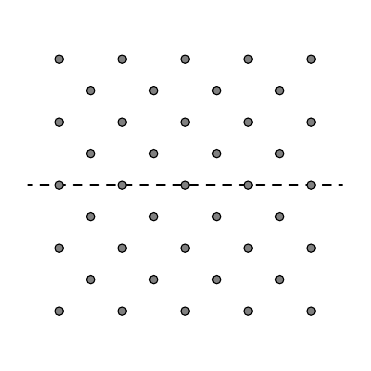
\begin{tikzpicture}[line cap=round,line join=round,>=triangle 45,x=0.8cm,y=0.8cm]\clip(-0.5,-0.5) rectangle (4.5,4.5);\draw [line width=0.6pt,domain=-1.8801411349281567:5.73722094225949,dashed] plot(\x,{(--8-0*\x)/4});
\begin{scriptsize}\draw [fill=gray] (0,0) circle (1.5pt);\draw [fill=gray] (1,0) circle (1.5pt);\draw [fill=gray] (2,0) circle (1.5pt);\draw [fill=gray] (3,0) circle (1.5pt);\draw [fill=gray] (4,0) circle (1.5pt);\draw [fill=gray] (4,1) circle (1.5pt);\draw [fill=gray] (3,1) circle (1.5pt);\draw [fill=gray] (2,1) circle (1.5pt);\draw [fill=gray] (1,1) circle (1.5pt);\draw [fill=gray] (0,1) circle (1.5pt);\draw [fill=gray] (0,2) circle (1.5pt);\draw [fill=gray] (1,2) circle (1.5pt);\draw [fill=gray] (2,2) circle (1.5pt);\draw [fill=gray] (3,2) circle (1.5pt);\draw [fill=gray] (4,2) circle (1.5pt);\draw [fill=gray] (4,3) circle (1.5pt);\draw [fill=gray] (3,3) circle (1.5pt);\draw [fill=gray] (2,3) circle (1.5pt);\draw [fill=gray] (1,3) circle (1.5pt);\draw [fill=gray] (0,3) circle (1.5pt);\draw [fill=gray] (0,4) circle (1.5pt);\draw [fill=gray] (1,4) circle (1.5pt);\draw [fill=gray] (2,4) circle (1.5pt);\draw [fill=gray] (3,4) circle (1.5pt);\draw [fill=gray] (4,4) circle (1.5pt);\draw [fill=gray] (0.5,0.5) circle (1.5pt);\draw [fill=gray] (0.5,1.5) circle (1.5pt);\draw [fill=gray] (1.5,1.5) circle (1.5pt);\draw [fill=gray] (1.5,0.5) circle (1.5pt);\draw [fill=gray] (2.5,0.5) circle (1.5pt);\draw [fill=gray] (3.5,0.5) circle (1.5pt);\draw [fill=gray] (3.5,1.5) circle (1.5pt);\draw [fill=gray] (2.5,1.5) circle (1.5pt);\draw [fill=gray] (2.5,2.5) circle (1.5pt);\draw [fill=gray] (3.5,2.5) circle (1.5pt);\draw [fill=gray] (3.5,3.5) circle (1.5pt);\draw [fill=gray] (2.5,3.5) circle (1.5pt);\draw [fill=gray] (1.5,3.5) circle (1.5pt);\draw [fill=gray] (0.5,3.5) circle (1.5pt);\draw [fill=gray] (0.5,2.5) circle (1.5pt);\draw [fill=gray] (1.5,2.5) circle (1.5pt);\end{scriptsize}\end{tikzpicture}}

\title{The Birch and Swinnerton-Dyer conjecture explained}
\author{TCC course by Raymond van Bommel}
\date{May--June 2025}

\begin{document}

\maketitle

These are notes for a hybrid course I taught as part of the Taught Course Centre (TCC).
Comments, questions and suggestions for correction and clarification are always welcome. 


\setcounter{tocdepth}{1}
\tableofcontents

\section{Introduction}

Let~$E$ be an elliptic curve defined over~$\Q$.
Then a famous theorem proved by Mordell in 1922 asserts the abelian group of rational points~$E(\Q)$ of~$E$ is finitely generated, i.e., it is of the shape
$$E(\Q) \cong T \times \Z^r,$$
where~$T$ is the finite torsion subgroup and the integer~$r$ is called the {\em (algebraic) rank} of~$E$, or~$\mathrm{rk}(E)$.
Even though it is known exactly which finite groups~$T$ can occur as the torsion subgroup (Mazur's theorem), less is known about the rank. It is conjectured, but not proved, that the rank is 0 for~$50\%$ of elliptic curves and 1 for another~$50\%$ of elliptic curves and greater than 1 for infinitely many but~$0\%$ of elliptic curves:
$$\lim_{X \to \infty} \frac{\#\{ E \mid H(E) \leq X \textrm{ and } \mathrm{rk}(E) = r \}}{\#\{ E \mid H(E) \leq X\}} = \begin{cases}\tfrac12 &\textrm{if } r \in \{0 , 1\}\\ 0 &\textrm{else}\end{cases},$$
where~$H(E) = \max(4|A|^3, 27B^2)$ is the height of the elliptic curve~$E \colon y^2 = x^3 + Ax + B$ written in minimal Weierstra\ss\ form.
There is no consensus on whether there exist a uniform bound for the rank of all elliptic curves over~$\Q$.
An elliptic curve with rank at least 29 has been found in 2024, breaking the previous record of 28 from 2006.
It would actually be very hard to prove that this elliptic curve has rank exactly 29; techniques (descent) to prove such things might be discussed later in this course.

On the other hand, changing the equations of~$E$ if needed, we can assume that~$A$ and~$B$ are integers and minimal, and we can reduce the equation modulo~$p$ to obtain a curve~$E_p$ over~$\F_p$.
For all but finitely of the primes~$p$, the curve~$E_p$ will also be a (smooth) elliptic curve, and~$E$ is said to have {\em good reduction} at~$p$.
For the other primes,~$E$ has either {\em multiplicative reduction} if~$E_p$ has a node, or {\em additive reduction} if~$E$ has a cusp.
Moreover, the multiplicative reduction is called {\em split} if the tangent directions of the curve at the node are rational, and {\em non-split} otherwise.

Hasse's theorem states that~$$|\# E_p(\F_p) - (p+1)| \leq 2\sqrt{p}$$ for all primes~$p$ of good reduction.
We define~$a_p = p+1 - \#E_p(\F_p)$ and
$$L_p(T) = \begin{cases}
1 - a_pT + pT^2 &\textrm{if~$p$ is a prime of good reduction},\\
1 - T &\textrm{if~$p$ is a prime of split multiplicative reduction},\\
1 + T &\textrm{if~$p$ is a prime of non-split multiplicative reduction},\\
1   &\textrm{if~$p$ is a prime of additive reduction}.
\end{cases}$$
We then define the~$L$-function of~$E$ as
$$L(E,s) = \prod_p L_p(p^{-s}).$$
The function~$L(E,s)$ extends\footnote{This is actually very non-trivial to prove and follows from the modularity theorem.} to an analytic function~$\C \to \C$ and it the order of the vanishing at 1 is called the {\em analytic rank} of~$E$, or~$\rkan(E)$.

\begin{conjecture}[Birch--Swinnerton-Dyer]
$$\mathrm{rk}(E) = \rkan(E)$$
\end{conjecture}

The conjecture does not only predict the order of vanishing of the~$L$-function at 0, but it also predicts the leading coefficient of the Taylor series at~$s = 1$.
The version below is the general version for abelian varieties~$A$ over a number field~$K$.

\begin{conjecture}[\textrm{BSD over~$\Q$, \cite[Conj.\ F.4.1.6, p.\ 462]{HindrySilverman}}]
Let~$A/\Q$ be an abelian variety of dimension~$d$ and algebraic rank~$r$. Let~$L(A,s)$ be its~$L$-function,~$A^{\vee}$ its dual,~$R_A$ its regulator,~$\Sh(A)$ its Tate-Shafarevich group and~$P_A$ its period. For each prime~$p$, let~$c_p$ be the Tamagawa number of~$A$ at~$p$.
Then~$L(A,s)$ has a zero of order~$r$ at~$s = 1$ and~\begin{equation}\label{eq:BSD}\lim_{s \rightarrow 1} {(s-1)^{-r} L(A,s)} = \frac{P_AR_A \cdot |\Sh(A)| \cdot \prod_{p} c_p}{|A(\Q)_{\tors}| \cdot |A^\vee(\Q)_{\tors}|}.\end{equation}
\end{conjecture}

In this course, we will study the different invariants occurring in the formula, approaches to compute them, and their relation to other important subjects in arithmetic geometry.
Sometimes we will focus on the case when~$A$ is the Jacobian~$J$ of a curve~$C$.

\section{Abelian varieties}

The topic of abelian varieties is so vast that one can fill a whole course with it.
I will try to highlight some of the things we will need about abelian varieties and refer you to the literature for the full theory.
A good source is the unpublished book \cite{AbVarBook}.

\begin{definition}[abelian variety]
An {\em abelian variety} over a field~$k$ is a proper/complete variety~$A$ over~$k$ that also carries a group structure. That is, there is a multiplication~$m \colon A \times A \to A$, an identity element~$e \colon \{ \star \} \to A$ and an inverse~$i \colon A \to A$ satisfying the usual group axioms.
\end{definition}

\begin{fact}
The group structure on an abelian variety is automatically commutative. The proof is omitted.
\end{fact}

\begin{example}[\textrm{\cite[Example 1.10]{AbVarBook}}]
Let~$C$ be a (hyperelliptic) curve of genus 2 over~$k$.
Then~$C$ has a hyperelliptic involution~$i \colon C \to C$.
Consider the surface~$$C^{(2)} \coloneqq (C \times C) / \iota,$$ where~$\iota \colon C \times C \to C \times C$ swaps the two coordinates.
The antidiagonal~$$\Delta^{-} \coloneqq \{ (P, i(P)) : P \in C\}/\iota \quad \subset \quad C^{(2)}$$
turns out to be a curve of genus 0 with self-intersection~$-1$ and by the theory of algebraic surfaces there exists a contraction/blow-down~$C^{(2)} \to J$ which contracts~$\Delta^{-}$ to a point and is an isomorphism outside of~$\Delta^{-}$.

On the other hand, it is known for the genus 2 curve~$C$ that the divisor~$P + i(P)$ is in the canonical divisor class for any~$P \in C$.
This can be used to construct a map~$$J(k) \to \mathrm{Cl}^0(C) \colon \quad (P,Q) \mapsto [P + Q - K_C],$$ where~$\mathrm{Cl}^0(C)$ is the the group of divisors on~$C$ of degree 0 modulo principal divisors.
It follows from the Riemann-Roch theorem that this map is a bijection, and we can use this bijection to supply~$J$ with a group structure and therefore the structure of an abelian variety.

The abelian variety~$J$ is the {\em Jacobian} of~$C$.
\end{example}

\begin{remark}
More generally, for a curve~$C$ of genus~$g$, the Jacobian~$J$ of~$C$, representing the group~$\mathrm{Pic}^0(C)$ line bundles of degree 0 on~$C$, is an abelian variety, and if~$C$ has a~$k$-rational point, then~$J$ is birational to~$C^{(g)}$.
\end{remark}

\begin{definition}[dual abelian variety]
For an abelian variety~$A$ the {\em dual abelian variety}~$A^\vee$ is the identity component~$\mathrm{Pic}^0(A)$ of the variety~$\mathrm{Pic}(A)$ representing the group of isomorphism classes of line bundles on~$A$.
\end{definition}

In general, the dual abelian variety~$A^{\vee}$ is isogenous to~$A$, i.e.\ there is a surjective map~$A \to A^{\vee}$ with finite kernel. For Jacobians the situation is better.

\begin{proposition}
Let~$J$ be the Jacobian of a curve over~$k$. Then~$J^\vee$ is isormorphic to~$J$.
\end{proposition}

\begin{proof}[Sketch of proof]
Reduce to the case that there is a~$k$-rational point~$P$ of~$C$.
Then the image of the map~$$C^{(g-1)} \to C^{(g)} \sim J \colon \quad (P_1, \ldots, P_{g-1}) \mapsto (P_1, \ldots, P_{g-1}, P)$$ gives a divisor~$\Theta \subset J$.
Then the map~$$\varphi_{\Theta} \colon J \to J^\vee \colon \quad x \mapsto t_x^* \Theta \otimes \Theta^{-1},$$ where~$t_x \colon J \to J$ is the translation-by-$x$ map, turns out to be an isomorphism.17:31
Details can be found in \cite[Chapter 14]{AbVarBook}
\end{proof}

\begin{corollary}
If~$A$ is the Jacobian of a curve, then the factors~$|A(\Q)_{\mathrm{tors}}|$ and~$|A^{\vee}(\Q)_{\mathrm{tors}}|$ in the BSD formula are equal.
\end{corollary}

\begin{definition}[Poincar\'e bundle]
The line bundle on $A \times A^\vee$ corresponding to the identity map~$A^\vee \to A^\vee$ is called the {\em Poincar\'e bundle} $\mathcal{P}$.
\end{definition}

For those not aware what this means, you can think like this.
Every point~$x \in A^\vee$ corresponds to a line bundle~$\mathcal{L}$ on~$A$.
If you restrict $\mathcal{P}$ to $A \times \{x\}$, you get the line bundle~$\mathcal{L}$.
So the Poincar\'e bundle is some way to glue all the line bundles on~$A$ into a large line bundle.

\begin{remark}
The Poincar\'e bundle can also be used to show that $A^{\vee\vee} \cong A$.
\end{remark}


\section{Models of curves and abelian varieties}

The book \cite{Liu} is a good place to read more about the topic.

Let~$K$ be a global or local field, e.g.\ a number field, or a finite extension of the field~$\mathbb{Q}_p$ of~$p$-adics. Let~$\mathfrak{p}$ be a prime of the ring of integers~$\mathcal{O}$ of~$K$ and let~$\mathcal{O}_\mathfrak{p}$ be the localisation of~$\mathcal{O}$ at~$\mathfrak{p}$.

The following definition is for people who are familiar with the language of schemes.

\begin{definition}[model of a curve]
Let~$C$ be a curve over~$K$. Then {\em a model of~$C$ over~$\mathcal{O}_\mathfrak{p}$} is a normal, proper, flat~$\mathrm{Spec}(\mathcal{O}_\mathfrak{p})$-scheme~$\mathcal{C}$, such that all fibres are pure of dimension 1, together with an isomorphism between the generic fibre~$\mathcal{C}_{\eta}$ and the curve~$C$.
\end{definition}

For those not familiar with this language follows a sketch of what this means. Suppose we start with a curve over~$\Q$ and~$p$ is a prime. Then to get a model, we need to make sure that the following holds.\footnote{These properties are not a formally correct definition, but rather indicate the kind of properties we need.}\\[-0.7cm]
\begin{itemize}\itemsep0pt
\item The coefficients of the defining equations of the curve do not have~$p$s in the denominators.
\item When you reduce the equation modulo~$p$, you get a curve. This curve can have isolated singularities, but cannot have a whole component that is singular (e.g.,~$y^2 = p\cdot x$ would not be allowed).
\item If you take a point in~$C(\Q)$, then it can be reduced modulo~$p$ to a unique point in~$\mathcal{C}(\F_p)$ (also for extensions of~$\Q$).
\end{itemize}

\subsection{Regular models}

\begin{definition}[regular points/scheme]
Let~$X$ be a scheme. Then a point~$p \in X$ is called {\em regular} if the maximal ideal~$\mathfrak{m}_p \subset \mathcal{O}_{X,p}$ can be generated by~$\dim(\mathcal{O}_{X,p})$ elements, or equivalently when the vector space~$\mathfrak{m}_p / \mathfrak{m}_p^2$ has dimension~$\dim(\mathcal{O}_{X,p})$.

The scheme~$X$ is said to be {\em regular} is it is regular at every point.
\end{definition}

\begin{fact}
Under some technical conditions, which are satisfied in the case of models of curves, the non-regular locus is a closed subset of~$X$. 
\end{fact}

\begin{example}\label{ex:non-reg-pt}
Consider the model~$\mathcal{C} \colon y^2 = x^5 + x^2 + p^2$ over~$\Z_{(p)}$.
The point~$P = (0,0)$ in the special fibre~$\mathcal{C}_{\F_p}$ corresponds to the maximal ideal~$\mathfrak{m}_{P} = (x,y,p)$ in the local ring~$$\left(\Z_{(p)}[x,y] / (y^2 - x^5 - x^2 - p^2)\right)_{(x,y,p)}.$$
The ideal~$\mathfrak{m}_{P}$ cannot be generated by 2 element. The reason is that the elements~$\overline{x}, \overline{y},$ and~$\overline{p}$ are linearly independent in~$\mathfrak{m}_P / \mathfrak{m}_P^2$, because all the terms in the equation lie in~$\mathfrak{m}_P^2$. Therefore~$\mathcal{C}$ is not regular at~$P$.
\end{example}

\begin{figure}[h]
\centering
\includegraphics[width=6cm]{blowup.png}
\caption{An illustration of a blow up, picture by Hauser}
\end{figure}

For some of the BSD-invariants of~$\mathrm{Jac}(C)$, we need to have a regular model of~$C$. Luckily, such models always exist and can be obtained by repeatedly blowing up non-regular points.

\begin{example}
In the set-up of Example~\ref{ex:non-reg-pt}, we will blow up~$\mathcal{C}$ at the point~$P$.
We introduce new projective coordinates~$U, V,$ and~$T$ and satisyfing the relations~$$Uy = Vx, \qquad Up = Tx, \qquad Vp = Ty.$$
This blow up has three charts.
For the first chart ``$U = 1$'', we get the relations~$y = vx$, and~$p = tx$, where~$v = \frac{V}{X}$ and~$t = \frac{T}{X}$. The equation of the curves changes into
$$x^2v^2 - x^5 - x^2 - x^2t^2 = 0, \qquad p = tx.$$
We will divide by~$x^2$, to remove the exceptional locus of the blow up and obtain
$$v^2 - x^3 - 1 - t^2 = 0, \qquad p = tx.$$
In the special fibre of this chart, we already see two components: they are given by~$t = 0$ and~$x = 0$, respectively.
The first component is a smooth curve of genus 1, and the second component is a smooth curve of genus 0.
In this chart, the components intersect at~$(v,t,x) = (\pm 1, 0 , 0)$.

%For the second chart ``$V = 1$'', we obtain the equations
%$$1 - u^5y^3 - u^2 - t^2, \qquad p = ty,$$
%and for the third chart ``$T = 1$``, we obtain the equations
%$$v^2 - u^5p^3 - u^2 - 1.$$

Note that compared to blow-ups of varieties over fields, the number of variables is increasing, as we cannot ``replace all~$p$ by~$tx$''.
\end{example}

\begin{theorem}[Lipman]
A regular model is obtained after finitely many blow-ups.
\end{theorem}

\begin{remark}
There are other ways to construct regular models of curves. For example, for hyperelliptic curves cluster pictures can be used, see \cite{HyperUser}, and for some plane curves, see \cite{Deltavregular}. These methods, although way more conceptual and pleasant to use, do not work for all curves.
\end{remark}

\subsection{(Semi-)stable models}

\begin{definition}[(semi-)stable curve]
A curve~$C$ is said to be {\em (semi-)stable} of genus~$g \geq 2$ if\\[-0.7cm]
\begin{itemize}\itemsep0pt
\item~$C$ is geometrically reduced and geometrically connected;
\item all singularities of~$C$ are nodes / ordinary double points;
\item each component of geometric genus 0 meets the other components in at least (two) three points;
\item~$\dim(H^1(\mathcal{O}_C)) = g$.
\end{itemize}\mbox{}\\[-0.7cm]
A model~$\mathcal{C}$ of a smooth curve~$C$ of genus at least 2 over~$K$ is said to be {\em (semi-)stable} if its special fibre if semi-stable.
\end{definition}

Not every smooth curve has a (semi-)stable model, but this is true after a finite extension.

\begin{theorem}[Deligne-Mumford, (semi)-stable reduction theorem]
There exists a finite extension~$L$ of~$K$ and an extension~$\mathfrak{q}$ of the prime~$\mathfrak{p}$ such that the base change~$C_L$ has a (semi-)stable model over~$\mathcal{O}_{L,\mathfrak{q}}$. 
\end{theorem}

\subsection{\texorpdfstring{N\'eron models}{Néron models}}

A good source to learn more about all the technicalities around N\'eron models is the book \cite{BLR}.

Let~$A$ be an abelian variety over~$K$. There does not always exist a model~$\mathcal{A}/\mathcal{O}_K$ such that the special fibre~$\mathcal{A}_{\mathbb{F}_\mathfrak{p}}$ is also an abelian variety, e.g.\ take an elliptic curve with bad reduction. The N\'eron model is in some sense the closest you can get without losing the group structure.

\begin{definition}[N\'eron model]
A {\em N\'eron model} of~$A$ at~$\mathfrak{p}$ is a smooth separated~$\mathcal{O}_{K,\mathfrak{p}}$-scheme~$\mathcal{A}$ that has the following {\em N\'eron mapping property}: for any smooth separated~$\mathcal{O}_{K,\mathfrak{p}}$-scheme~$X$, any morphism~$X_K \to A$ on the generic fibre extends uniquely to a morphism~$X \to \mathcal{A}$ over~$\mathcal{O}_{K, \mathfrak{p}}$.
\end{definition}

As a consequence of the definition of a N\'eron model, the group structure on~$A$ given by the multiplication map~$m \colon A \times A \to A$, the identity map~$e \colon \{\star\} \to A$ and the inverse map~$i \colon A \to A$, extends to the N\'eron model~$\mathcal{A}$, giving it a group structure. Another consequence of the defintition is that the N\'eron model is unique, if it exists.

\begin{theorem}[N\'eron]
Every abelian variety has a N\'eron model.
\end{theorem}

N\'eron models are typically not proper, as the N\'eron mapping property is weaker than the valuative criterion for properness.
It is does follow from the definition, however, that there is a reduction map on rational points~$A(K) \to \mathcal{A}(\mathcal{O}_{K,\mathfrak{p}})$.

\begin{example}
Let~$E$ be an elliptic curve and~$\mathcal{E}$ its minimal regular model (i.e.\ a regular model on which no components can be contracted).
Then the smooth locus of~$\mathcal{E}$ is a N\'eron model of~$E$. We consider four cases:\\[-0.7cm]
\begin{itemize}\itemsep0pt
\item If~$E$ has good reduction, then~$\mathcal{E}_{\F_\mathfrak{p}}$ is the reduction of~$E$, which is an elliptic curve.
\item If~$E$ has split multiplicative reduction, then~$\mathcal{E}_{\F_\mathfrak{p}}$ is a ``circle of~$\mathbb{P}^1$s'', and the special fibre of the N\'eron model is of the shape~$\mathbb{G}_{\mathrm{m}} \times \Z/n\Z$ for some integer~$n$.
\item If~$E$ has non-split multiplicative reduction, then it is split multiplicative after an extension. The special fibre of the N\'eron model consists of copies of~$\mathbb{G}_{\mathrm{m}, \mathbb{F}_{\mathfrak{p}^2}}$ that are permuted by Galois and non-split tori. Here~$\mathbb{F}_{\mathfrak{p}^2}$ denotes the quadratic extension field of~$\mathbb{F}_{\mathfrak{p}}$.
\item In the case of additive reduction, the special fibre N\'eron model is of the shape~$\mathbb{G}_{\mathrm{a}} \times \Phi$, where~$\Phi$ is a finite group of order at most 4.
\end{itemize}
\end{example}

\begin{fact}
The N\'eron model is not stable under base change! Indeed, if an elliptic curve has additive reduction, we know that it will obtain good or multiplicative reduction over some finite extension, so the N\'eron model must change.
\end{fact}

In the case of a curve~$C$ over~$K$ and its Jacobian~$J$, the N\'eron model~$\mathcal{J}$ is related to regular or semi-stable models~$\mathcal{C}$ of~$C$.

\begin{theorem}
Let~$\mathcal{C}$ and~$\mathcal{J}$ be as above. Assume (in the case of a regular model), that the greatest common divisor of the multiplicities of the irreducible components in the special fibre is equal to 1. Then the Picard scheme~$\mathrm{Pic}^0_{\mathcal{C}/\mathcal{O}_{K,\mathfrak{p}}}$ coincides with the identity component~$\mathcal{J}^0$ of~$\mathcal{J}$.
\end{theorem}

\section{Period}

\subsection{For abelian varieties}

Let~$A$ be an abelian variety of dimension~$g$ over a number field~$K$, and let~$\sigma \colon K \hookrightarrow \C$ be an embedding into the complex numbers. Then
$$A_\sigma \coloneqq A \times_\sigma \C \stackrel{\textrm{as complex manifold}}{\cong} \C^g / \Lambda$$
for some lattice~$\Lambda$.

The periods of~$A_\sigma$, i.e.\ the generators of the lattice~$\Lambda$, can be found by integrating a basis of differentials~$\underline{\omega} = (\omega_1, \ldots, \omega_g)$ of~$\Omega^1_A(A)$ inside~$\Omega^1_{A_\sigma}(A_\sigma)$ along a set of generators~$(\gamma_1, \ldots, \gamma_{2g})$ of the homology group~$H^1(A_{\sigma}, \Z)$:
\begin{equation}\label{eq:lambda}\Lambda \sim \Z \begin{pmatrix} \int_{\gamma_1} \omega_1 \\ \vdots \\\int_{\gamma_1} \omega_g\end{pmatrix} \oplus \cdots \oplus \Z \begin{pmatrix} \int_{\gamma_{2g}} \omega_1 \\ \vdots \\\int_{\gamma_{2g}} \omega_g\end{pmatrix}.\end{equation}

Note that the lattice that you get this way depends on the choice of the basis~$\underline{\omega}$ of~$\Omega^1_{A}(A)$.
By changing the basis, one changes the~$\C$-basis of the vector space~$\C^g$.

We first define the complex period.

\begin{definition}[local complex period]
Suppose that~$\sigma$ is a complex place, i.e.\ that~$\sigma$ does not map~$K$ into~$\R$.
Then the {\em local period of~$A$ at~$v$ with respect to~$\underline{\omega}$} is
$$\Omega_{A,\sigma, \underline{\omega}} = \left|\det \left(\int_{\gamma_i} \omega_j, \overline{\int_{\gamma_i} \omega_j}\right)_{i,j=1}^{i=2g,j=g}\right|.$$
\end{definition}

In the real case, the real period measure the size of the lattice~$\Lambda \cap \R^g$.
Below there are two examples of lattices corresponding to elliptic curves.
In the picture, complex conjugation corresponds to reflection through the central horizontal line.
The other dotted line in the right hand picture represents the second real component.
The real period measures the distance between two nodes on the dotted line (up to a factor 2).

\begin{figure}[h]
\centering
\latttwee \qquad \latteen
\caption{Examples of lattices in~$\C$ with one (left) and two (right) real components.}
\end{figure}

\begin{definition}[local real period]
Suppose that~$\sigma \colon K \hookrightarrow \R$ is a real place.
Let~$(\gamma_1', \ldots, \gamma_g')$ be a basis of~$H^1(A_\sigma(\C), \Z)^{\mathrm{Gal}(\C/\R)}$ and let~$m_\sigma$ be the number of connected components of~$A_\sigma(\R)$. Then the {\em local period of~$A$ at~$v$ with respect to~$\underline{\omega}$} is
$$\Omega_{A,\sigma, \underline{\omega}} = m_v \cdot \left|\det\left(\int_{\gamma_i'} \omega_j\right)_{i,j=1}^g\right|.$$
\end{definition}

Note that the product~$$\Omega_{A,\underline{\omega}} \coloneqq \prod_{\sigma} \Omega_{A,\sigma,\underline{\omega}}$$
still depends on the choice of~$\underline{\omega}$. 
To resolve this problem and to get a well-defined quantity, we let~$\mathcal{A} / \mathcal{O}_K$ be a N\'eron model of~$A$ over~$\mathcal{O}_K$.

\begin{definition}[period]\label{def:period}
Suppose~$\underline{\omega}$ is an~$\mathcal{O}_K$-basis of the module~$\Omega^1_{\mathcal{A}/\mathcal{O}_K}(\mathcal{A})$ of global relative differentials on~$\mathcal{A}$. Then the {\em period} of~$A$ is defined to be~$\Omega_{A,\underline{\omega}}$ as above.
\end{definition}

\begin{remark}
The sheaf of relative differentials~$\Omega^1_{\mathcal{A}/\mathcal{O}_K}$, as defined in \cite[Sect.~6.1]{Liu}, is a sheaf that `glues' the usual sheaves of differentials~$\Omega^1_{A/K}$ on the generic fibre and~$\Omega^1_{\mathcal{A}_{\mathfrak{p}}/\mathbb{F}_{\mathfrak{p}}}$ on the special fibres of~$\mathcal{A}$.

The~$\mathcal{O}_K$-module~$\Omega^1_{\mathcal{A}/\mathcal{O}_K}(\mathcal{A})$ does not need to be a free module (c.f.\ a non-principal ideal inside~$\mathcal{O}_K$ when~$K$ has class number greater than 1). The module is only guaranteed to be locally free, and Definition~\ref{def:period} can be fixed by taking any~$\underline{\omega}$ and measuring how far~$\underline{\omega}_\mathfrak{p}$ is from being a basis of~$\Omega^1_{\mathcal{A}_{\mathfrak{p}}/\mathbb{F}_{\mathfrak{p}}}(\mathcal{A}_\mathfrak{p})$, see also \cite[Subsect.~1.3.4]{PhD}.
\end{remark}

\subsection{For Jacobians}

For a curve~$C$ over a number field~$K$, it is also possible to obtain the periods of its Jacobian~$J$ directly from the curve.
Let~$\underline{\omega} = (\omega_1, \ldots, \omega_g)$ be a basis of differentials of~$\Omega_C^1(C)$.
For any embedding~$\sigma \colon K \hookrightarrow \C$, we can consider these differentials as elements of~$\Omega^1_{C_\sigma}(C_\sigma)$ and integrate them along a set of generators~$(\gamma_1, \ldots, \gamma_{2g})$ of the homology~$H^1(C_\sigma, \Z)$ and create a lattice as in Equation~\eqref{eq:lambda}.

We will now describe which differentials correspond to those in~$\Omega^1_{\mathcal{J}/\mathcal{O}_K}(\mathcal{J})$. For this purpose, we introduce the canonical sheaf. The following definitions can also be found in~\cite[Sect.~6.4]{Liu}.

\begin{definition}[determinant]
Let~$X$ be a scheme, and let~$\mathcal{F}$ be a locally free~$\mathcal{O}_X$-module of rank~$r$.
Then we define~$\det \mathcal{F}$ to be the line bundle~$\wedge^r \mathcal{F}$, i.e.\ on any affine open~$U\subset X$ we let~$(\det \mathcal{F})(U) = \wedge^r M$, where~$M$ is the~$\mathcal{O}_X(U)$-module such that~$\mathcal{F}|_U \cong \widetilde{M}$.
\end{definition}

The canonical sheaf as defined below is a generalisation of the line bundle~$\det \Omega^1_{X/T}$ for smooth schemes~$X$ over~$T$.

\begin{definition}[canonical sheaf]
Let~$Y/T$ be a quasi-projective locally noetherian scheme that is a local complete intersection (e.g.~$Y$ is a semi-stable or regular model of a curve over~$T = \mathrm{Spec}(\mathcal{O}_K)$). Let~$i \colon Y \to Z$ be an immersion into a smooth scheme~$Z/T$ (e.g.\ projective space).
Then the {\em canonical sheaf} of~$Y/T$ is the~$\mathcal{O}_Y$-module
$$\omega_{Y/T} \coloneqq \det(i^*(\mathcal{I}/\mathcal{I}^2))^\vee \otimes_{\mathcal{O}_T} i^*(\det \Omega^1_{Z/T}),$$
where~$\mathcal{I}$ is the sheaf of ideals defining~$Y$ in an open~$Z' \subset Z$ containing~$Y$ as closed subset.
\end{definition}

\begin{remark}
This is independent of the choice of~$Z$ and~$i$, see~\cite[Sect.~6.4]{Liu}.
Moreover, the canonical sheaf is stable under base change, see~\cite[Thm.~6.4.9]{Liu}, and for a smooth~$Z/T$, it coincides with~$\det \Omega_Z^1$, see~\cite[Cor.~6.4.13]{Liu}.
\end{remark}

To get some idea what this canonical sheaf is, we consider the case of a semi-stable curve.

\begin{theorem}[\textrm{\cite[Prop.~13.2.9]{Olsson}}]
Let~$C$ be a semi-stable curve over a field~$k$ and let~$\pi \colon \widetilde{C} \to C$ the normalisation.
Let~$D = \sum_{y \in \pi^{-1}(C_{\mathrm{sing}})} [y]$ be the divisor on~$C'$ consisting of the points that need to be glued on~$C'$ to obtain~$C$.
Then there is an exact sequence
$$0 \to \omega_{C/k} \to \pi_*\Omega^1_{\widetilde{C}}(D) \to \bigoplus_{P \in C_{\mathrm{sing}}} k(P).$$
In other words, the sections of~$\omega_{C/k}$ correspond to differentials on~$\widetilde{C}$ that are allowed to have simple poles at the points in~$D$ such that for any~$P \in C_\mathrm{sing}$ the sum of the residues at the poles corresponding to the two points in~$\pi^{-1}(P)$ is zero.
\end{theorem}

\begin{example}
Take a ``nodal elliptic curve''~$C$, i.e.\ glue~$\widetilde{C} = \mathbb{P}^1$ at the points~$0$ and~$\infty$.
On~$\widetilde{C}$, we have~$\Omega^1_{\widetilde{C}}([0] + [\infty]) \cong \mathcal{O}_{\widetilde{C}}(2 - 2) \cong \mathcal{O}_{\widetilde{C}}$.
The differential~$\frac1x\,dx$ has simple poles at~$0$ and~$\infty$.
The residue at~0 is~1, and writing the differential as~$-x\,d\frac{1}{x}$, we see that the residue at~$\infty$ is~$-1$.
Therefore, as their sum is zero\footnote{The sum of the residues of such a differential is always 0, so in this case it was not necessary to check that. It does become non-trivial when there are more points to glue.}, the differential gives rise to a global section of~$\omega_{C/k}$.
\end{example}

We turn back to the problem of finding the correct differentials for the period.

\begin{lemma}[\textrm{\cite[Lem.~1.3.5]{PhD}}]
Let~$\mathcal{C}$ be a regular model\footnote{For this theorem, it would actually be enough to consider a model with at most rational singularities.} of~$C$ over~$\mathcal{O}_{K,\mathfrak{p}}$, and let~$\mathcal{J}$ be a N\'eron model over~$\mathcal{O}_{K,\mathfrak{p}}$ of the Jacobian of~$C$.
Then there is an isomorphism~$\Omega^1_{\mathcal{J}/\mathcal{O}_{K,\mathfrak{p}}}(\mathcal{J}) \cong \omega_{\mathcal{C}/\mathcal{O}_{K,\mathfrak{p}}}(\mathcal{C})$.
\end{lemma}

Note that as the canonical sheaf is stable under base change, we have~$$\omega_{\mathcal{C}/\mathcal{O}_{K,\mathfrak{p}}}(\mathcal{C}) \otimes_{\mathcal{O}_{K,\mathfrak{p}}} K \cong \omega_{C/K}(C) \cong \Omega^1_C(C).$$
So we now see that the basis~$\underline{\omega}$ of~$\Omega^1_C(C)$ that we want to pick in order to find the period of~$J$, is one that corresponds to a basis of~$\omega_{\mathcal{C}/\mathcal{O}_{K,\mathfrak{p}}}(\mathcal{C})$.

\subsection{Periods and endomorphisms}

Any map $\varphi \colon A \to B$ from an abelian variety to another abelian variety such that $\varphi(0_A) = 0_B$, is automatically also an homomorphism of group varieties, i.e.\ $\varphi$ respects the group structure.

\begin{definition}[isogeny/simple AV/endomorphism algebra]
A morphism $\varphi \colon A \to B$ is called an {\em isogeny} if two of the three following properties hold:\\[-0.8cm]
\begin{itemize}\itemsep0pt
\item $\varphi$ is surjective;
\item $\dim(A) = \dim(B)$;
\item $\ker(\varphi)$ is finite.
\end{itemize}\mbox{}\\[-0.7cm]
The abelian varieties $A$ and $B$ are called {\em isogenous} if such a $\varphi$ exists, and we write $A \sim B$.
An abelian variety $A$ is called {\em simple} if $A \sim B \times C$ can only hold if either $B$ or $C$ is zero-dimensional.

The set of endomorphisms~$\mathrm{End}(A)$ is a ring with the composition of endomorphism as multiplication, and the ring $$\mathrm{End}^0(A) \coloneqq \mathrm{End}(A) \otimes_{\Z} \Q$$ is called the {\em endomorphism algebra} of $A$.
\end{definition}

Note that it is possible for an abelian variety $A$ over a field $K$ to be simple, and for $A_{\overline{K}}$ to not be simple. For example, if $L/K$ is a quadratic extension and $B$ is abelian variety over $L$ and $B^\sigma$ its conjugate, then $B \times B^\sigma$ could be isogenous (over $L$) to a simple abelian variety over $K$.

\begin{theorem}[\textrm{\cite[Corollary~12.7]{AbVarBook}}]
Let $A$ be an abelian variety such that
$$A \sim B_1^{e_1} \times \cdots \times B_n^{e_n}$$
for some simple abelian varieties $B_1, \ldots, B_n$ such that $B_i \not\sim B_j$ if $i \neq j$. Then
$$\mathrm{End}^0(A) \cong M_{e_1}(D_1) \times \cdots \times M_{e_n}(D_n),$$
where $D_i \coloneqq \mathrm{End}^0(B_i)$ is a division algebra, and $M_{\ell}(R)$ denotes the ring of $\ell \times \ell$-matrices with coefficients in $R$.
\end{theorem}

There is a more refined classification of the possibilities for the $D_i$ in the theorem above, which is called the Albert classification.
There are four possibilities:\\[-1.0cm]
\begin{itemize}\itemsep0pt
\item $D$ is a totally real field (type I),
\item $D$ split/Hamiltonian quaternion algebra over a totally real field (type II/III), 
\item $D$ is a central simple algebra over a CM field, i.e.\ a central simple algebra over a totally imaginary quadratic extension of a totally real field (type IV).
\end{itemize}

In the case of the Jacobian $J$ of a curve $C$, one can use correspondences to describe an endomorphism $J \to J$.

\begin{definition}[correspondence]
For (reasonable) varieties $X$ and $Y$, a correspondence between~$X$ and $Y$ is a closed subset $R$ of $X \times Y$. For convenience, we will assume that $R$ does not contain subsets of the form $\{x\} \times Y$ or $X \times \{y\}$ for any $x \in X$ or $y \in Y$.
\end{definition}

Suppose you have a divisor/correspondence $R \subset C \times C$, then this can describe an endomorphism~$J \to J$ as follows.
Let $D \in J = \mathrm{Pic}^0(C)$ be some divisor class $\sum_i n_i[P_i]$ on~$C$.
Then~$\{P_i\} \times C$ intersects $R$ in finitely many points $(P_i, Q_{ij})$, with multiplicity if needed, and we can define a map~$J \to J$ by
$$D = \sum_i n_i[P_i] \mapsto \sum_{i,j} n_i Q_{ij}.$$

The periods of $A$ can be used to (heuristically) determine the endomorphism ring/algebra of $A$.
Indeed, if we arrange the generators of the lattice $\Lambda$ in a $g \times 2g$-matrix $\Pi$ with entries in $\mathbb{C}$, then an endomorphism $A \to A$ gives rise to an equality
$$M\Pi = \Pi R,$$
where $M$ is a $g \times g$-matrix over $\C$, describing a homothety of the lattice, and $R$ is a $2g \times 2g$-matrix over $\Z$, describing the map of lattices. There are commonly used algorithms that solve this problem numerically in order to determine $\mathrm{End}(A)$, see \cite{endomorphisms}. It is possible to get certified output, for example in the form of a correspondence of a curve.

\section{Regulator}

\subsection{Heights on varieties}

In this section, we will define the regulator of an abelian variety over a number field. First, we need to discuss some generalities on heights. This is explained well in \cite{Lang} and \cite{Neron} (if you don't mind French).

\begin{definition}[standard height]
Let~$K$ be a number field. The {\em standard height on~$\P^n_K$} is defined by
$$h_{\P^n_K}  \colon \P^n_K(\overline{K}) \rightarrow \R \colon (x_0 : \cdots : x_n) \mapsto \frac{1}{[L:K]} \sum_{v \in M_L} [L_v : \Q_v] \log \max_{i = 0, \ldots, n} \{|x_i|_v\},$$
where~$L/K$ is a finite extension containing~$x_0, \ldots, x_n$, and~$M_L$ is the set of (finite and infinite) places\footnote{Finite place are prime ideals of $\mathcal{O}_L$ and infinite places are embeddings of $L$ into $\R$ or $\C$. Places correspond to the non-trivial absolute values you can put on $K$.} of~$L$, and where for all finite places~$v$ over the prime~$p \in \Z$ the absolute value~$| \cdot |_v$ is normalised such that~$|p|_v = p^{-1}$.
\end{definition}

\begin{example}
Over~$\Q$, for a rational point~$(x_0 : \cdots : x_n)$ with~$x_0, \ldots, x_n \in \Z$ coprime, we have~$$h_{\mathbb{P}^n_{\Q}}(x_0 : \cdots : x_n) = \log\max(|x_0|, \ldots, |x_n|).$$
\end{example}

For the rest of this section, let~$X/K$ be smooth and projective over a number field~$K$.

\begin{definition}[na\"ive height]
Let~$\mathcal{L}$ be a very ample line bundle on~$X$ and let~$\mathcal{B}$ be an ordered basis of its global sections, giving rise to an immersion~$\varphi \colon X \rightarrow \P^n_K$. Then we can define the {\em na\"ive global height of~$X$ at~$\mathcal{L}$ with respect to~$\mathcal{B}$} as
$$h_{X,\mathcal{L},\mathcal{B}}^{\textrm{naive}}\colon X(\overline{K}) \rightarrow \R \colon P \mapsto h_{\P^n_K}(\varphi(P)).$$
\end{definition}

We will now try to extend this definition to work for all line bundles in~$A$. For this purpose we will define the following space.

\begin{definition}[height function space]
Let~$\textrm{Map}(X(\overline{K}), \R)$ be the~$\R$-vector space of all functions from~$X(\overline{K})$ to~$\R$. Let~$\textrm{Map}^0(X(\overline{K}), \R)$ be the subspace of these functions that are bounded, i.e.\ the~$f \colon X(\overline{K}) \to \R$ for which there exists a~$B \in \R$ such that~$|f(P)| < B$ for all~$P \in X(\overline{K})$. Then the {\em height function space} of~$X$ is~$$\mathcal{H}(X) := \mathrm{Map}(X(\overline{K}), \R) \, / \, \mathrm{Map}^0(X(\overline{K}), \R).$$
\end{definition}

Now we can extend the definition of the global height of~$X$ to also work at line bundles~$\mathcal{L}$, which are not necessarily very ample.

\begin{lemma}[\textrm{\cite[Thm.\ 5.1, sect.\ 4.5, p.\ 93]{Lang}}]\label{thm:heightPic}
There exists a function~$$h_{A, \cdot} \colon \Pic(A) \rightarrow \mathcal{H}(X) \colon [\mathcal{L}] \mapsto h_{X,[\mathcal{L}]},$$ having the following properties:\\[-0.8cm]
\begin{itemize}\itemsep0pt
\item[--] for~$[\mathcal{L}_1], [\mathcal{L}_2] \in \Pic(X)$ we have~$h_{X,[\mathcal{L}_1]} + h_{X,[\mathcal{L}_2]} = h_{X,[\mathcal{L}_1 \otimes \mathcal{L}_2]}$;
\item[--] if~$\mathcal{L}$ is a very ample line bundle and~$\mathcal{B}$ an ordered basis of its global sections then~$h_{X,[\mathcal{L}]}$ is the class of~$h_{X,\mathcal{L},\mathcal{B}}^{\mathrm{naive}}$.
\end{itemize}
Moreover, this construction is functorial in the following sense. If~$f \colon X \rightarrow Y$ is a morphism of smooth projective schemes over~$K$ and~$\mathcal{L}$ is a line bundle on~$Y$, then~$h_{X, [f^*\mathcal{L}]} = h_{Y, [\mathcal{L}]} \circ f$. 
\end{lemma}

\subsection{Canonical height on an abelian variety}

In case of abelian varieties, for such height functions, there is a canonical representative in the set~$\mathrm{Map}(A(\overline{K}), \R)$. Just like for elliptic curves (for those who already heard of the height in that situation), the height can be seen as a measure for how many digits you need to write down a point.

\begin{proposition}[\textrm{\cite[Thm.\ 5, sect.\ II.14, p.\ 300]{Neron}}]
Let~$\mathcal{L}$ be a line bundle on an abelian variety~$A$ over~$K$. Then there exist functions~$\ell, q \colon A(\overline{K}) \rightarrow \R$, that are linear and quadratic (i.e.~$q(P + Q) - q(P) - q(Q)$ is a bilinear form on~$A(\overline{K}) \times A(\overline{K})$), respectively, such that~$\ell+q$ is in the class~$h_{A,[\mathcal{L}]}$.
\end{proposition}

\begin{proof}[Sketch of proof]
Let $(-1) \colon A \to A$ be the multiplication by $-1$. Let $\mathcal{M} = (-1)^*\mathcal{L}$. Then $[\mathcal{L}] + [\mathcal{M}]$ is a so-called symmetric line bundle, and the limit $$\lim_{N \to \infty} \frac{h_{X,[\mathcal{L}] + [\mathcal{M}]}^\textrm{naive}(NP)}{N^2}$$
exists, giving rise to the quadratic part $q$. On the other hand, $[\mathcal{L}] - [\mathcal{M}]$ is anti-symmetric, and in this case the limit $$\lim_{N \to \infty} \frac{h_{X,[\mathcal{L}] - [\mathcal{M}]}^\textrm{naive}(NP)}{N}$$ exists, giving rise to the linear part $\ell$.
\end{proof}

\begin{remark}
While the limit in the proof above, gives you a good way to think about the height, this limit does not give a very fast way to compute the height in practice.
\end{remark}

\begin{definition}[canonical height]
For a line bundle~$\mathcal{L}$ on an abelian variety~$A$ with functions~$\ell, q \colon A(\overline{K}) \rightarrow \R$ as above, we define the {\em canonical height of~$A$ at~$\mathcal{L}$} as~$$\widehat{h}_{A,\mathcal{L}} = \ell + q.$$
\end{definition}

\begin{fact}
For an ample $\mathcal{L}$, the set $\bigcup_{[L:K] \leq d} \{ x \in A(L) : \widehat{h}_{A,\mathcal{L}}(x) \leq B\}$ is finite for any $B$ and $d$ (Northcott property). Moreover, the only points of height 0 are torsion points.
\end{fact}

The above definition of height depends on the choice of a line bundle $\mathcal{L}$. To get an even more canonical notion of height, we consider $A \times A^\vee$.

\begin{definition}[N\'eron-Tate height]
Let~$\mathcal{P}$ be the Poincar\'e bundle on~$A \times A^{\vee}$. Then the {\em N\'eron-Tate height on~$A$} is defined as
$$h_{A \times A^{\vee},\, \textrm{NT}} = \widehat{h}_{A \times A^{\vee}, \mathcal{P}}  : A(\overline{K}) \times A^{\vee}(\overline{K}) \rightarrow \R.$$
\end{definition}

Now we can define the regulator of $A$.

\begin{definition}[regulator]
Let~$P_1, \ldots, P_{\mathrm{rk}(A)}$ be a basis of the free part of~$A(\Q)$, Moreover, let~$Q_1, \ldots, Q_{\mathrm{rk}(A)}$ be a basis of the free part of~$A^\vee(\Q)$. Then the {\em regulator} of~$A$ is defined as
$$\left|\det\!\begin{pmatrix}
h_{A \times A^{\vee},\, \textrm{NT}}(P_1, Q_1)   &\cdots     &h_{A \times A^{\vee},\, \textrm{NT}}(P_{\mathrm{rk}(A)}, Q_1)\\
\vdots  &\ddots     &\vdots \\
h_{A \times A^{\vee},\, \textrm{NT}}(P_1, Q_{\mathrm{rk}(A)})   &\cdots     &h_{A \times A^{\vee},\, \textrm{NT}}(P_{\mathrm{rk}(A)}, Q_{\mathrm{rk}(A)})
\end{pmatrix}\right|.$$
\end{definition}

\subsection{Canonical height for Jacobians using Arakelov intersection theory}

Let $J$ be the Jacobian of a curve $C$ over a number field $K$.
Then as $J^\vee \cong J$, the height pairing becomes a function $J(\overline{K}) \times J(\overline{K}) \to \R$.
Instead of trying to compute on $J$ directly, it is actually possible to express the heights using arithmetic and geometry information attached to the curve~$C$.

\begin{theorem}[Faltings-Hriljac]
Let $D,E$ be degree 0 divisors on $C$ with disjoint support. Then the N\'eron-Tate height can be expressed as a sum $$-\sum_{v \in M_K} \langle D, E \rangle_v,$$
where $M_K$ is the set of finite and infinite places of $K$, and $\langle \cdot, \cdot \rangle_v$ is a local intersection pairing, which we will roughly after this.
\end{theorem}

Let us now describe these local intersection pairings.
We first consider the case of a finite place, given by a prime ideal $\mathfrak{p} \subset \mathcal{O}_K$.
Let $\mathcal{C}$ be a regular model of $C$ over $\mathcal{O}_{K,\mathfrak{p}}$.
Then $\mathcal{C}$ just behaves like an algebraic surface over a field in the sense that you can do intersection theory on it.

\begin{definition}[horizontal/vertical divisors]
Let $D \subset \mathcal{C}$ be irreducible of codimension 1.
Then~$D$ is called {\em vertical}, if $D$ is contained in the special fibre $\mathcal{C}_\mathfrak{p}$, i.e.\ if $D$ is an irreducible component of $\mathcal{C}_\mathfrak{p}$.
If $D$ is not vertical, then $D$ is called {\em horizontal}, in which case $D$ consists of a point in the generic fibre $\mathcal{C}_{\eta} \cong C$ together with the reduction modulo $\mathfrak{p}$ of that point in $\mathcal{C}_\mathfrak{p}$.

Divisors are called horizontal/vertical if their support consists of horizontal/vertical subschemes.
\end{definition}

\begin{definition}[intersection number] \label{def:intersection}
Let $D_1, D_2 \subset \mathcal{C}$ be irreducible and distinct.
Then $D_1 \cap D_2$ is finite, and for each point $P \in D_1 \cap D_2$, we can define the intersection multiplicity at $P$ as
$$\iota_{P}(D_1, D_2) \coloneqq \mathrm{length}_{\mathcal{O}_{\mathcal{C},P}}\!\left( \frac{\mathcal{O}_{\mathcal{C},P}}{\mathcal{I}_{D_1,P} + \mathcal{I}_{D_2,P}}\right),$$
where $\mathcal{I}_{D_1,P}$ and $\mathcal{I}_{D_2,P}$ are ideals defining $D_1$ and $D_2$ respectively.
We then define the {\em intersection number}
$$\iota(D_1,D_2) \coloneqq \sum_{P \in D_1 \cap D_2} \iota_P(D_1,D_2) \cdot \log|k_P|,$$
where $k_P$ is the (finite) field of definition of $P$.
This function can be extended bilinearly to pairs of divisors with disjoint support.
\end{definition}

\begin{remark}
If you intersect two horizontal irreducibles corresponding to points $P_1, P_2 \in C$, then you are essentially computing the highest power $\mathfrak{p}^i$ of $\mathfrak{p}$ such that $P_1$ and $P_2$ are congruent modulo $\mathfrak{p}^i$.
If you intersect a horizontal and a vertical irreducible, corresponding to a point $P \in C$ and a component $D \subset \mathcal{C}_\mathfrak{p}$, you are determining whether the reduction of $P$ lies on $D$.
\end{remark}

\begin{remark}
There are a lot of subtleties with this intersection pairing.
If $D$ is a vertical divisor, and if we consider the whole special fibre $\mathcal{C}_\mathfrak{p}$ as a divisor, then we can extend the intersection pairing by setting $\iota(D, \mathcal{C}_\mathfrak{p}) = 0$, and use this to determine $\iota(D,D)$.
Note that this does not hold for horizontal divisors, as $\iota(D, \mathcal{C}_\mathfrak{p}) \neq 0$ in this case, unless $D$ has degree 0 on $C$.
\end{remark}

Now we can define the local pairing $\langle D, E \rangle_\mathfrak{p}$.

\begin{definition}
Let $D$ and $E$ be divisors on $C$ of degree 0.
Let $\overline{D}$ and $\overline{E}$ be the horizontal divisors on $\mathcal{C}$ corresponding to $D$ and $E$.
We define
$$\langle D, E \rangle_\mathfrak{p} \coloneqq \iota\!\left( \overline{D} + \Phi(\overline{D}), \overline{E} + \Phi(\overline{E})\right),$$
where $\Phi(\overline{D})$ (and similarly $\Phi(\overline{E})$) is a vertical divisor such that $\iota(Y, \overline{D} + \Phi(\overline{D})) = 0$ for all vertical divisors $Y$.\footnote{It is not a priori clear that this vertical divisor $\Phi(\overline{D})$ exists, see \cite{Arakelov,heights}.}
\end{definition}

For the infinite places $v$ of $K$, the pairing $\langle D, E\rangle_v$ can be defined using the Riemann theta function corresponding to $\C^g / \Lambda$. The details are omitted and can be found in \cite{Arakelov,heights}.

\section{Tate-Shafarevich group}

\subsection{\texorpdfstring{Torsors, twists and $H^1$}{Torsors, twists and H1}}

In arithmetic geometry, there are often situations where two objects are not isomorphic but become isomorphic after base changing to an algebraic closure.
Examples of such objects are twists and torsors of abelian varieties. This topic is also discussed in \cite[Chap.~X]{SilvermanBook}.

\begin{definition}[twist]
Let $A$ and $B$ be abelian varieties over a field $K$.
Then $B$ is said to be a {\em twist} of $A$ if $A_{\overline{K}} \cong B_{\overline{K}}$.
\end{definition}

\begin{definition}[torsor]
Let $A$ be an abelian variety over a field~$K$, and let $X$ be a variety over~$K$ with an action of $A$ on it, i.e.\ a map $A \times X \to X$, satisfying the usual properties.
Then~$X$ is called an {\em $A$-torsor}, or principal homogeneous space, if $X_{\overline{K}}$ is isomorphic to $A_{\overline{K}}$, as a variety with an action of $A_{\overline{K}}$.

An $A$-torsor $X$ is called {\em trivial} if $X \cong A$, or equivalently if $X(K) \neq \emptyset$.
\end{definition}

\begin{example}\label{ex:torsor}
Let $C$ be the curve given by $3x^3 + 4y^3 + 5z^3 = 0$ in $\P^2$ over $\Q$.
This is a famous example of a genus 1 curve without a rational point.
The Jacobian $E$ of $C$ is an elliptic curve, and $E$ carries a natural action $E \times C \to C$.
The curve $C$ is an $E$-torsor under that action.
\end{example}

The set of twists or torsors, up to isomorphism over $K$, can be expressed as a cohomology set.
We will first state the theorem and then explain it more in the rest of the subsection.

\begin{theorem}\label{thm:h1}
Let $A$ be an abelian variety over a number field $K$. Let $G_K = \mathrm{Gal}(\overline{K}/K)$ be the absolute Galois group of $K$. Then there are isomorphisms
$$\{ \textrm{twists of } A\} /_{\cong_K} \cong H^1(G_K, \mathrm{Aut}(A_{\overline{K}})),$$
$$\{ A\textrm{-torsors}\} /_{\cong_K} \cong H^1(G_K, A_{\overline{K}}).$$
\end{theorem}

The pattern that you will see is that the group on the right is the automorphism group of the object in question after base changing to $\overline{K}$.
Indeed, for $A_{\overline{K}}$ considered as a variety with an action of $A_{\overline{K}}$ on it, the automorphisms consist of translations by points in $A_{\overline{K}}$.

There are other examples of this phenomenon.
For example, line bundles, which become trivial when you look at small enough open subsets, are classified by $H^1(X, \mathbb{G}_\mathrm{m})$ or $H^1(X, \mathcal{O}_X^*)$.
In this case, $\mathbb{G}_\mathrm{m}$ is the automorphism group of a trivial line bundle.
Another example is that of central simple algebras, which can be classified using cohomology sets like $H^1(G_K, \mathrm{PGL}_n)$.

The general setup for $H^1(G, A)$ is that $G$ is a group acting on a group $A$.
In our case, $G$ is the absolute Galois group acting on the automorphisms over $\overline{K}$ by acting on the coefficients occurring in the automorphisms.

The reason $H^1(G,A)$ exists, is because the functor $A \mapsto A^G$ mapping the group to its invariance, is not exact. 
If $A$ is abelian, then there is a whole theory of homological algebra, which will give cohomology sets $H^n(G,A)$ with long exact sequences, et cetera.
For this course, I will only give a definition for $H^1(G,A)$ that also works for non-abelian $A$, and you will have to consult other sources for more background on the general theory, e.g.\ \cite[App.~B]{SilvermanBook}.
Note that $H^1(G,A)$ will not be a group, but only a pointed set, unless $A$ is abelian.

\begin{definition}
Let $G$ be a group acting on another group $A$, we will denote this action by ${}^ga$ for $g \in G$ and $a \in A$.
A {\em cross morphism} is a map $f \colon G \to A$ such that
$$f(g_1g_2) = f(g_1) \cdot {}^{g_1}f(g_2), \qquad \textrm{for all $g_1,g_2 \in G$.}$$
Two cross morphisms $f_1$ and $f_2$ are called {\em cohomologous} if there is an $a \in A$ such that $$f_2(g) = a^{-1} \cdot f_1(g) \cdot {}^ga, \qquad \textrm{for all $g \in G$.}$$
The {\em cohomology set} $H^1(G,A)$ is the set of cross morphisms modulo the equivalence of cohomologous cross morphisms.
\end{definition}

\begin{proof}[Idea of proof of Theorem~\ref{thm:h1}]
Consider an $A$-torsor $X$ over $K$ (the situation of twists is analogous). Let $i \colon A_{\overline{K}} \to X_{\overline{K}}$ be an isomorphism. For any $\sigma \in G_K$, the composite map
$$\xymatrix{A_{\overline{K}} \ar[r]^{{}^\sigma i} &X_{\overline{K}} \ar[r]^{i^{-1}} &A_{\overline{K}},
}$$
where ${}^\sigma i$ is the isomorphism you get by applying $\sigma$ to the coefficients of $i$, is translation by an element $a_{\sigma}$.
You can now check that the map $\sigma \mapsto a_{\sigma}$ is a cross morphism.

The other way around, if you are given a cross morphism $f$, then this can be used to construct a torsor.
The idea is to consider the variety $A$ over $K$ as a variety over $\overline{K}$ with the action of~$\mathrm{Gal}(\overline{K}/K)$ on it, and change this action action of the Galois group.
More specifically, any element $\sigma \in \mathrm{Gal}(\overline{K}/K)$ gives rise to a map $\sigma_A \colon A_{\overline{K}} \to A_{\overline{K}}$ (over $K$, not over $\overline{K}$).
This action of Galois can be twisted by replacing $\sigma_A$ with $f(\sigma) \circ \sigma_A$.
Then one can use descent on $A_{\overline{K}}$ with this new Galois action to get another variety $X$ over $K$, the $A$-torsor.
\end{proof}

We will demonstrate the construction for twists by the means of an example.

\begin{example}
Let $E \colon y^2 = f(x)$ be an elliptic curve over $\Q$. Let $$f \colon \mathrm{Gal}\!\left(\overline{\Q}/\Q\right) \to \mathrm{Gal}\!\left(\Q\left(\sqrt{d}\right)\!/\Q\right) \to \mathrm{Aut}\!\left(E_{\overline{\Q}}\right)$$ be the cross morphism that maps the non-trivial element of $\mathrm{Gal}(\Q(\sqrt{d})/\Q)$ to the automorphism~$-1 \colon (x,y) \mapsto (x, -y)$, and the identity to the identity.
Then the twisted Galois action on~$E$ is given by
$$\left(a + b\sqrt{d}\right) \cdot x \quad \mapsto \quad \left(a - b\sqrt{d}\right) \cdot x,$$
$$\left(a + b\sqrt{d}\right) \cdot y \quad \mapsto \quad \left(-a + b\sqrt{d}\right) \cdot y.$$
The ring of invariants under this action is generated by $x' = x$ and $y' = \sqrt{d}\cdot y$, and we see that they will satisfy the relation $y'^2 = d \cdot f(x')$.
In other words, we get the quadratic twist.
\end{example}

\begin{remark}
Note that the quadratic twist could be isomorpic to $E$ itself.
This may happen if~$\mathrm{Aut}(E_{\overline{\Q}})$ has more than 2 elements, and the cross morphism will actually become homologous to the cross morphism mapping everything to the identity.
\end{remark}

\subsection{Local-global principle for torsors}

Now we are ready to define the Tate-Shafarevich group.

\begin{definition}[Tate-Shafarevich group]
Let $A$ be an abelian variety over a number field $K$.
Let $M_K$ be the set of places of $K$.
Then the {\em Tate-Shafarevich group} of $A$ is the group
$$\Sh(A/K) \coloneqq \bigcap_{v \in M_K} \ker\!\left(H^1(G_K, A_{\overline{K}}) \to H^1(G_{K_v}, A_{\overline{K_v}})\right),$$
where $K_v$ is the completion of $K$ at $v$, and $\ker(\cdots)$ is the set of elements mapping to the trivial torsor.
\end{definition}

In other words, $\Sh(A/K)$ is the set of torsors $X$ of $A$ such that $X$ has a point over $K_v$ for all places $v$, up to isomorphism over $K$.
These are torsors that have point everywhere locally, but not necessarily globally.
You could say that $\Sh(A/K)$ measures the failure of the local-global principle for torsors of abelian varieties.

\begin{example}
The torsor from Example~\ref{ex:torsor} corresponds to a non-trivial element of the Tate-Shafarevich group of the Jacobian $E$ occurring in that example.
This element turns out to have order 3.
\end{example}

\begin{remark}
While it is conjectured that $\Sh(A/K)$ is finite, this is not proved.
It is known that $\Sh(A/K)[n]$ is finite, but that doesn't exclude the possibility of $\Sh(A/K)$ containing some infinite divisible group like $\Q$.

If $\Sh(A/K)_\textrm{div}$ is the maximal divisible subgroup of $\Sh(A/K)$, then it has been believed for a long time that~\ $|\Sh(A/K)/\Sh(A/K)_\textrm{div}|$ would be a square. The reason for that is that there is a pairing, called the {\em Cassels-Tate pairing}
$$\langle \cdot, \cdot \rangle \colon \Sh(A/K) \times \Sh(A^\vee/K) \to \Q/\Z,$$
and this pairing was believed to be alternating after mapping $\Sh(A/K)$ to $\Sh(A^\vee/K)$ through some polarisation, i.e.\ $\langle x,x \rangle = 0$.
If the polarisation is principal, the pairing can be shown to be antisymmetric, i.e.\ $\langle x,y\rangle = -\langle y,x\rangle$, which is a weaker property.
It turns out that the pairing is not alternating in general and even for Jacobians $J$ the order $|\Sh(J/K)/\Sh(J/K)_\textrm{div}|$ can also be two times a square, see also \cite{PoonenStoll}.


\end{remark}

\subsection{Descent and Selmer groups}

\subsubsection{Setup}

This subsection gives an introduction to descent and Selmer groups.
For a more complete picture of the theory, you could read \cite{descent} or \cite[Chap.\ X]{SilvermanBook}.
Let us start with the elliptic curve
$$E \colon y^2 = x(x-a)(x-b) \textrm{ over } \Q.$$
For a rational point $(x,y) \in E(\Q)$, the numbers $x, x-a,$ and $x-b$ do not need to be squares, but their product should be.
Let us do a substitution
$$x = d_1 x_1^2, \quad x-a = d_2 x_2^2, \quad x-b = d_1d_2 x_3^2, \quad y = d_1d_2d_3 x_1x_2x_3.$$
This naturally leads to the curve
$$C_{d_1,d_2} \colon \quad d_1x_1^2 = d_2x_2^2 + a = d_1d_2x_3^2 + b.$$
There is a natural map
$$\varphi_{d_1,d_2} \colon C_{d_1,d_2} \to E \colon \quad (x_1, x_2, x_3) \mapsto (d_1x_1^2, d_1d_2d_3x_1x_2x_3).$$
Any rational point on $E(\Q)$ must come from a rational point on $C_{d_1,d_2}(\Q)$ for some choice of $d_1$ and $d_2$.
So suppose you want to find generators of the Mordell-Weil group $E(\Q)$, then it could be useful to study rational points on $C_{d_1,d_2}$.

\subsubsection{Covers as twists}

The cover $\varphi_{d_1,d_2}$ is unramified, and $\mathrm{Aut}(C_{d_1,d_2}/E) = \Z/2\Z \times \Z/2\Z \cong E[2]$, given by the maps $$(x_1,x_2,x_3) \mapsto (\pm x_1, \pm x_2, \pm x_3)$$ with an even number of plus signs.
Note that different curves $C_{d_1,d_2}$ and $C_{d_1',d_2'}$ become isomorphic over $\overline{\Q}$: they are twists.
In this case, the group $\Q^*/\Q^{*2} \times \Q^*/\Q^{*2}$ classifies these twists.
In light of what we learned before, it would not be hard to believe the following more general statement.

\begin{proposition}
The $E[2]$-covers of $E$ are classified by the group $H^1(G_{\Q}, E[2])$.
\end{proposition}

Note that any point $(x,y) \in E(\Q)$ is the image of a rational point on some $C_{d_1,d_2}$. Indeed, we need $d_1 = x \in \Q^* / \Q^{*2}$ and $d_2 = x - a \in \Q^*/\Q^{*2}$. This gives a natural map
$$\rho \colon E(\Q) \to H^1(G_\Q, E[2]) : (x,y) \mapsto C_{d_1,d_2}.$$

\begin{remark}
Another way to get this map is by taking the long exact sequence of group cohomology for the exact sequence of algebraic groups $0 \to E[2] \to E \stackrel{\cdot 2}{\to} E \to 0$. Doing it this way, you'll see that $\rho$ factors through $E(\Q) / 2E(\Q)$.
\end{remark}

\subsubsection{Local-global principle again}

If you want to know if $C_{d_1,d_2}$ has rational points, you might as well first consider if $C_{d_1,d_2}$ has points everywhere locally, i.e.\ over every completion $\Q_v$ of $\Q$.
It turns out that the curve $C_{d_1,d_2}$ only has points everywhere locally for finitely many of the possible values of $d_1$ and $d_2$.

We want to determine these $d_1$ and $d_2$.
For our $C_{d_1,d_2}$, it turns out that $d_1$ and~$d_2$ are only allowed to have prime factors that occur in $2ab(a-b)$ if we want $C_{d_1,d_2}(\Q_v) \neq \emptyset$ for all places $v$.
For the general case, this motivates the following definition.

\begin{definition}[Selmer group]
Let $A$ be an abelian variety over a number field $K$ and let $n$ be an integer\footnote{Instead of integers, it is also possible to use other endomorphisms of $A$, in the case $\mathrm{End}(A) \neq \Z$.}. Then the {\em $n$-Selmer group} $\mathrm{Sel}_n(A)$ is the subgroup of those $H^1(K, A[n])$ whose restriction to $H^1(K_v, A[n])$ lies in the image of the local map $\rho_v \colon A(K_v) \to H^1(G_{K_v}, A[n])$ for every place $v$ of $K$.
\end{definition}

In other words, the Selmer groups classifies $A[n]$-covers of the abelian variety that have points everwhere locally.
As we know, having points everywhere locally is not a guarantee for having a point globally.
The failure is again measured by the Tate-Shafarevich group.

\begin{lemma}
There is an exact sequence
$$0 \to A(K)/nA(K) \to \mathrm{Sel}_n(A) \to \Sh(A/K)[n] \to 0.$$
\end{lemma}

\begin{proof}
The proof is omitted, but follows from an analysis of a bunch of long exact sequences.
\end{proof}

\begin{fact}
The Selmer group is finite and, in principle, effectively computable.
The idea is that group~$H^1(K,E[n])$ can be embedded in $R^* / R^{*,n}$, where $R$ is a product of fields over which the points in $E[n]$ are defined.
The most difficult step in computing the Selmer group is the computation of the class and unit groups of these fields. Again, see \cite{descent} for more background.

As a consequence of this fact, the Selmer group can be used to bound the rank of $E$ and~$\Sh(E/K)[n]$.
If you believe that $\Sh(E/K)$ is finite, then there must be an $n$ for which the right term of the sequence is 0, and you will actually find a sharp upper bound of the rank.
On the other hand, there is no unconditional algorithm known to compute the rank of an elliptic curve.
\end{fact}

\section{Tamagawa number}

Let $\mathcal{A}$ be a N\'eron model over $\mathcal{O}_{K,\mathfrak{p}}$ of an abelian variety $A$ over a number field $K$ at a prime $\mathfrak{p}$ of~$K$.
The special fibre $\mathcal{A}_{\mathfrak{p}}$ over the residue field $k_\mathfrak{p}$ does not need to be connected.
The connected component containing the identity element $\mathcal{A}_\mathfrak{p}^0$ is a subgroup, and the quotient $\Phi \coloneqq \mathcal{A}_{\mathfrak{p}} / \mathcal{A}_\mathfrak{p}^0$ is called the component group.

\begin{definition}[Tamagawa number]
The {\em Tamagawa number} of $A$ at $\mathfrak{p}$ is defined to be $$c_{\mathfrak{p}} \coloneqq \#\Phi(k_\mathfrak{p}).$$
\end{definition}

Let $K_\mathfrak{p}$ be the completion of $K$ at $\mathfrak{p}$.
For elliptic curves $E$ with a minimal Weierstra\ss\ equation, the Tamagawa number is sometimes also defined as $\# (E(K_\mathfrak{p}) / E(K_\mathfrak{p})^0)$ where $E(K_\mathfrak{p})^0$ is the subgroup of points whose reduction is a smooth point (on the reduction of the minimal Weierstra\ss\ model).
The lemma below explains why this is the same.

\begin{lemma}
There is an equality $$c_\mathfrak{p} = \#\!\left( \mathcal{A}(K_\mathfrak{p}) / \mathcal{A}^0(K_\mathfrak{p})\right).$$
\end{lemma}

\begin{proof}
Let $R$ be the ring of integers in $K_\mathfrak{p}$.
By the N\'eron mapping property $\mathcal{A}(K_\mathfrak{p}) = \mathcal{A}(R)$.
This also induces a reduction map $\mathcal{A}(K_\mathfrak{p}) \to \mathcal{A}(R) \to \mathcal{A}_\mathfrak{p}(k_\mathfrak{p})$. This reduction map is surjective, because $\mathcal{A}$ is smooth and $K_\mathfrak{p}$ is complete (Hensel's lemma).
Moreover, as $\mathcal{A}^0$ is open, the reduction maps $\mathcal{A}^0(K_\mathfrak{p})$ into $\mathcal{A}_\mathfrak{p}^0(k_\mathfrak{p})$, and the kernel of $\mathcal{A}(K_\mathfrak{p}) \to \Phi(k_\mathfrak{p})$ is $\mathcal{A}^0(K_\mathfrak{p})$.
\end{proof}

Note that the Tamagawa number is 1 for all primes of good reduction.
In particular, only finitely many of the $c_\mathfrak{p}$ are not equal to 1.

\begin{remark}
There is a different notion of Tamagawa numbers for reductive algebraic groups.
While this notion shows similarity to the one for abelian varieties, they should not be considered the same.
In fact, historically, the Tamagawa numbers for elliptic curves have been called fudge factors.
The exact definition of these fudge factors was determined later, see for example \cite{Tate}.
\end{remark}

\subsection{For Jacobians}

In the case of a Jacobian $J$ of a curve $C$ over a number field $K$, the Tamagawa number $c_\mathfrak{p}$ can be determined using intersection theory on regular model $\mathcal{C}$ over $\mathcal{O}_{K,\mathfrak{p}}$.

Let $I$ be the set of geometrically irreducible components of the special fibre $\mathcal{C}_{k_\mathfrak{p}}$.
Let $L$ be an unramified extension of $K$ over, and let $\mathfrak{q}$ be a prime of~$L$ extending $\mathfrak{p}$, such that all components in $I$ are defined over $k_\mathfrak{q}$.
We define the intersection of two such components $D$ and $E$ as $$\langle D, E \rangle = \iota(D,E) / \log(k_\mathfrak{q}),$$ where $\iota$ is as in Def.~\ref{def:intersection}, so that $\langle D, E \rangle \in \Z$.
The component group of $\Phi$ can now be related to the intersections on the regular model as follows.

\begin{theorem}[\textrm{\cite[Thm.~1.1]{BoschLiu}}]
There is an exact sequence of $\mathrm{Gal}(k_\mathfrak{q}/k_\mathfrak{p})$-modules
$$0 \to \mathrm{im}(\alpha) \to \mathrm{ker}(\beta) \to \Phi(k_\mathfrak{q}) \to 0,$$
where $\alpha \colon \Z^I \to \Z^I$ is the linear map which maps a component $D \in I$ to $\sum_{E \in I} \langle D, E \rangle \cdot E \in \Z^I$, and~$\beta \colon \Z^I \to \Z$ is the linear map mapping a component $D \in I$ to its multiplicity in $\mathcal{C}_{k_\mathfrak{q}}$.
\end{theorem}

\begin{proof}[Proof sketch]
The N\'eron model $\mathcal{J}$ of $J$ is almost equal to the subfunctor of $\mathrm{Pic}_{\mathcal{C}/\mathcal{O}_{k_\mathfrak{q}}}$ consisting of divisor classes of total degree 0.
If you take a divisor $D$ of total degree 0 and some component~$E \in I$, then~$\langle D, E\rangle$ does not need to be 0, but the weighted sum of the $\langle D,E \rangle$ must be 0, as~$\mathcal{C}_{k_\mathfrak{q}}$ has intersection number 0 with every other divisor of total degree 0.
In other words, we get a map~$\mathrm{Div}^{0}_{\mathcal{C}/\mathcal{O}_{k_\mathfrak{q}}} \to \mathrm{ker}(\beta)$.
Moreover, the principal divisors correspond exactly to those in $\mathrm{im}(\alpha)$.
So we actually get a map~$\mathcal{J} \to \mathrm{ker}(\beta) / \mathrm{im}(\alpha)$.

The identity component $\mathcal{J}_\mathfrak{p}^0$ corresponds to those line bundles that have degree 0 on each component in $I$.
So now we have a map~$\mathcal{J}_\mathfrak{p}/\mathcal{J}_\mathfrak{p}^0 \to \mathrm{ker}(\beta) / \mathrm{im}(\alpha)$.
One then needs to show that this map is surjective, and respects the action of the Galois structure.
This is all a bit technical and can be found in \cite{BoschLiu, BLR}.
\end{proof}

\section{L-function}

\subsection{Definitions}

Let $A$ be an abelian variety over a number field $K$ of dimension $g$.
Let $G = \mathrm{Gal}(\overline{K}/K)$ be the absolute Galois group of $K$.
We first define the Tate module as follows.

\begin{definition}[Tate module]
For a prime $\ell$, the {\em Tate-$\ell$-module} is the $G$-module defined by
$$T_{\ell}(A) = \lim_{n \in \Z_{>0}} A[\ell^n](\overline{K}),$$
i.e., its elements are sequences $(t_1, t_2, \ldots)$ of $t_i \in A[\ell^i](\overline{K})$ such that $\ell \cdot t_i = t_{i-1}$ for all $i \geq 2$.
\end{definition}

Because $A[\ell^n](\overline{K}) \cong (\Z/\ell^n\Z)^{2g}$, there is an isomorphism $T_\ell(A) \cong \Z_{\ell}^{2g}$ of groups.
We define $V_{\ell}$ to be the $G$-module $T_{\ell}(A) \otimes _{\Z_\ell} \Q_\ell$.
The dual $\Hom(V_{\ell}(A), \Q_\ell)$ also has a $G$-module structure:
$$g \cdot \varphi(-) = \varphi(g^{-1} \cdot -), \quad \textrm{for } \varphi \in \Hom(V_{\ell}(A), \Q_{\ell}).$$

Let $\mathfrak{p}$ be a prime of $K$ coprime to $\ell$ and fix an extension $\mathfrak{q}$ of $\mathfrak{p}$ to $\overline{K}$.
Let $I_\mathfrak{q} \subset G$ be the inertia group, i.e.\ the subgroup of $\sigma \in G$ fixing $\mathfrak{q}$ and acting trivially on the residue field $k_\mathfrak{q}$.
The Frobenius element of~$\mathrm{Gal}(k_\mathfrak{q} / k_\mathfrak{p})$ lifts to an element $\mathrm{Frob}_\mathfrak{q}$ in $G$, which is only unique up to elements in $I_\mathfrak{q}$.

\begin{definition}[Euler factor]
We define the {\em Euler factor} of $A$ at $\mathfrak{p}$ to be
$$P_\mathfrak{p} \coloneqq \mathrm{det}\!\left( 1 - \mathrm{Frob}_\mathfrak{q} \cdot T \mid \mathrm{Hom}( V_\ell(A), \Q_\ell)^{I_v}\right) \in \Q_\ell[T].$$
\end{definition}

\begin{remark}
The coefficients of this polynomial turn out to lie in $\Z$, and the polynomial does not depend on the choice of $\mathfrak{q}$, $\ell$ or $\mathrm{Frob}_\mathfrak{q}$, as long as $\ell$ is coprime to $\mathfrak{p}$.
\end{remark}

The $L$-function can now be defined in terms of these Euler factors.

\begin{definition}[L-function]
The {\em $L$-function} of $A$ is defined by
$$L(A, s) = \prod_{\mathfrak{p}} P_\mathfrak{p}\!\left( (\# k_\mathfrak{p})^{-s}\right)^{-1}.$$
\end{definition}

A priori, one can show relatively easy that this gives rise to a holomorphic function on the space~$\{z \in \C : \mathrm{Im}(z) > \tfrac32\}$.
It is expected that it extends to a holomorphic function on $\C$.

\begin{conjecture}
The $L$-function can be continued to an a holomorphic function $\C \to \C$. Moreover, let
$$\Lambda(A,s) = \mathrm{Norm}(N)^{s/2} \cdot \left( (2\pi)^{-s} \, \Gamma(s) \right)^{g \cdot [K:\Q]} \cdot |\Delta(K)|^{g \cdot s} \cdot L(A,s),$$
where $N$ is the conductor of $A$ (to be defined later), $\Gamma(s)$ is the usual $\Gamma$-function, and $\Delta(K)$ the discriminant of $K$.
Then we have $$\Gamma(A, 2-s) = \varepsilon \cdot \Gamma(A,s) \quad \textrm{for all } s \in \C$$
where $\varepsilon \in \{\pm 1\}$ is the root number of $A$, i.e.\ $(-1)^{\mathrm{rk}(A) \bmod 2}$.
\end{conjecture}

One could say that the (norm of the) conductor is the integer that makes the functional equation work; this is what people sometimes call the {\em analytic conductor}.
There is also an algebraic definition of the conductor (and conjecturally this is the same).

\begin{definition}[Conductor, \textrm{\cite{BrumerKramer}}]
Let $A$ be an abelian variety over a number field $K$.
Let~$\mathfrak{p}$ be a prime of $K$ and let $\ell$ be a prime of $\Z$ coprime to $\mathfrak{p}$.
Consider $V_{\ell}(A)$ with the action of~$\mathrm{Gal}(\overline{K}_\mathfrak{p} / K_\mathfrak{p})$.
Then the {\em tame conductor exponent} of $A$ at $\mathfrak{p}$ is
$$\varepsilon(A,\mathfrak{p}) \coloneqq 2g - \dim\!\left(V_\ell(A)^I\right),$$
where $I$ is the inertia subgroup.

Moreover, if $L = K_\mathfrak{p}(A[\ell])$, then the {\em wild/Swan conductor exponent} of $A$ at $\mathfrak{p}$ is
$$\delta(A,\mathfrak{p}) \coloneqq \sum_{i=1}^\infty \frac{|G_i|}{|G_0|} \dim\!\left( A[\ell] / A[\ell]^{G_i} \right).$$
Here $G_i \subset \mathrm{Gal}(L / K_\mathfrak{p})$ is the $i$-th ramification group $$G_i \coloneqq \{ \sigma \in \mathrm{Gal}(L / K_\mathfrak{p}) : v_L( \sigma(\pi_L) - \pi_L) \geq i+1\},$$
where $\pi_L$ is a uniformiser of $L$ and $v_L$ is the discrete valuation on $L$.

The {\em conductor exponent} of $A$ at $\mathfrak{p}$ is defined as $f_\mathfrak{p} \coloneqq \varepsilon(A,\mathfrak{p}) + \delta(A,\mathfrak{p})$, and the {\em conductor} of~$A$ is then defined to be the ideal $\prod_\mathfrak{p} \mathfrak{p}^{f_\mathfrak{p}}$.
\end{definition}

\begin{fact}
If the residue characteristic $p$ of $\mathfrak{p}$ is greater than $2g + 1$, then the wild conductor exponent $\delta(A,\mathfrak{p})$ is equal to 0.
\end{fact}

\begin{remark}
It is also possible to define the Euler factors and the conductor using $H^1(A_{\overline{K}}, \Z_\ell)$ instead of $T_{\ell}(A)$, as there is a duality between the two groups, see \cite[Chap.\ 10]{AbVarBook}.
\end{remark}

\subsection{For Jacobians}

Let $C$ be a curve over a number field $K$ and let $J$ be its Jacobian.
Because $H^1(J_{\overline{K}}, \Q_\ell)$ is isomorphic to $H^1(C_{\overline{K}}, \Q_\ell)$, the computation of the Euler factors can also be done on the curve.
Consider a prime $\mathfrak{p}$ of good reduction and let $C_\mathfrak{p}$ be the reduction.
Then by the N\'eron-Ogg-Shafarevich criterion, the action of inertia on $H^1(J_{\overline{K}}, \Q_\ell)$ is trivial, and we need to compute the characteristic polynomial of Frobenius. This essentially comes down to computing the numerator of the zeta function
$$Z(C_\mathfrak{p}, T) \coloneqq \mathrm{exp}\!\left( \sum_{n = 1}^\infty \# C_\mathfrak{p}(k_{\mathfrak{p},n}) \cdot \frac{T^n}{n} \right),$$
where $k_{\mathfrak{p},n}$ is the degree $n$ extension field of the residue field $k_\mathfrak{p}$.
Because of the functional equation that the zeta function satisfies, it is sufficient to count points in $C_\mathfrak{p}(k_{\mathfrak{p},n})$ for $n = 1, \ldots, g$.

\begin{remark}
For elliptic curves, Schoof's algorithm can be used to count points in runtime that is polynomial in $\mathrm{log}(\# k_{\mathfrak{p}} )$.
For higher genus curves, there is no practical algorithm that does this in polynomial time.
However, if you want to compute the Euler factors for all $p \leq N$ at the same time, there are algorithms that can do that in average polynomial time, see for example \cite{HarveySutherland}.
\end{remark}

For the bad primes, there have been several strategies:\\[-0.9cm]
\begin{itemize}\itemsep0pt
\item try guessing the conductor exponents and Euler factors until you find a guess that satisfies the functional equation of the $L$-function;
\item compute the Euler factors on a regular model of $C$;
\item compute the Euler factors on the (semi)stable reduction of $C$.
\end{itemize}

We will go into more detail on the last two approaches. A good place to read more about this is~\cite{BouwWewers}.

\begin{lemma}[\textrm{\cite[Prop.\ 2.8]{BouwWewers}}]
Suppose that $\mathcal{C}$ is a regular or (semi-)stable model of $C$ over~$\mathcal{O}_{K,\mathfrak{p}}$.
Suppose that the greatest common divisor of the multiplicities of the components in the special fibre $\mathcal{C}_{k_{\mathfrak{p}}}$ is 1.
Then there is an isomorphism
$$H^1(C_{\overline{K}}, \Q_{\ell})^{I_K} \cong H^1(\mathcal{C}_{\overline{k}_\mathfrak{p}}, \Q_\ell).$$
\end{lemma}

It then turns out to be possible to determine the Euler factor by point counting on $\mathcal{C}_{\overline{k}_\mathfrak{p}}$, as the Euler factor is essentially the zeta function of $\mathcal{C}_{k_\mathfrak{p}}$.

As a regular model always exists without needing to extend the base field $K$, this method can always be applied in this case.
However, a regular model can be computationally expensive to compute.
There is also a way to use the stable reduction, even if $C$ does not have stable reduction over $K$.

Suppose that $L/K$ is a Galois extension, such that $C$ has stable reduction over $L$.
Let $\mathfrak{q}$ a prime of $L$ extending $\mathfrak{p}$, and let $\mathcal{C}$ be a stable model of $C$ over $\mathcal{O}_{L,\mathfrak{q}}$.
In \cite[Thm.\ 2.4]{BouwWewers}, it is proved that
$$H^1(C_{\overline{K}}, \Q_{\ell})^{I_K} \cong H^1(\mathcal{C}_{\overline{k}_\mathfrak{q}}, \Q_\ell)^{I_K} \cong H^1(\mathcal{C}_{\overline{k}_\mathfrak{q}} / I_{K}, \Q_{\ell}).$$

The Euler factor can now be determined by counting points on $\mathcal{C}_{k_\mathfrak{q}} \,/\, \mathrm{Gal}(L/K)$.
Moreover, the tame part of the conductor is
$$2 \cdot \mathrm{genus}(C) - \mathrm{genus}_{\mathrm{arith}}(\mathcal{C}_{\overline{k}_\mathfrak{q}} / I_{K}) - \mathrm{genus}_{\mathrm{geom}}(\mathcal{C}_{\overline{k}_\mathfrak{q}} / I_{K}).$$
For the wild part of the conductor, you also need to compute the genera of the curves $\mathcal{C}_{\overline{k}_\mathfrak{q}} / G_i$, where $G_i \subset I_{K}$ is the $i$-th ramification group, see also \cite[Thm.\ 2.9]{BouwWewers}.

\section{What is known about BSD?}

The most prominent result on the Birch and Swinnerton-Dyer conjecture is the statement that the conjecture holds for elliptic curves of analytic rank 0 and 1.
The proof, which is the accumulation of work by Gross-Zagier, Kolyvagin, and others, uses modularity, Heegner points, and Euler systems.
While there is not enough time in the course to discuss these in full detail, I will make an attempt to convey some of the ideas behind them.

There are also some other things known about the conjecture.
For example, it is known that the conjecture holds for an abelian variety $A$ over a number field $K$, if and only if it holds for an $K$-isogenous abelian variety, or in the case of a field extension $K/L$ for the Weil restriction~$\mathop{\mathrm{Res}_{K/L}} A$ of $A$.
In certain cases, there are also things known about the parity (odd/even) of the rank of an elliptic curve.
Finally, the conjecture can be viewed as a special case of the Bloch-Kato conjecture.

\subsection{Modularity}

Let $N$ be an intgeer.
There is an algebraic curve $Y_0(N)$ over $\Z[1/N]$ whose points correspond to pairs~$(E, \varphi \colon E \to E')$ of an elliptic curve $E$ together with an $N$-isogeny $\varphi$.
Complex analytically this corresponds to the quotient $\mathcal{H} / \Gamma_0(N)$, where $\mathcal{H}$ is the upper half plane $\{\mathrm{im}(z) > 0\}$, and
$$\Gamma_0 = \left\{ M \in \mathrm{SL}_2(\Z) : M \equiv  \begin{pmatrix}\star &\star\\ 0 &\star \end{pmatrix} \mod N \right\}.$$
This curve can be compactified into a projective curve $X_0(N)$ by also allowing ``generalised elliptic curves'', which are isomorphic to an $n$-gon of $\mathbb{P}^1$s.

\begin{theorem}[modularity theorem]
Let $E/\Q$ be an elliptic curve with conductor $N$.
Then there exists a surjective map $X_0(N) \to E$.
\end{theorem}

The modularity theorem, or Shimura-Taniyama conjecture, was proved first for semi-stable curves by Wiles and Taylor in 1995, as part of the proof of Fermat's last theorem, and later in full generality by Breuil, Conrad, Diamond, and Taylor in 2001.
As a consequence of the modularity theorem, the $L$-function of $E$ will be equal to the $L$-function of a certain modular form of weight~2, and we get the following.

\begin{corollary}
The $L$-function of $E$ extends to an analytic function $\C \to \C$.
\end{corollary}

\subsection{Heegner points}

Let $N$ be the conductor of an elliptic curve $E$ over $\Q$.
Let $K$ be an imaginary quadratic number field, such that every prime $p \mid N$ splits in $\mathcal{O}_K$.
Then there exists an ideal $\mathfrak{N}$ such that $$\mathcal{O}_K / \mathfrak{N} \cong \Z/N\Z.$$
Embedding $K$ into $\C$, we get an $N$-isogeny of elliptic curves over $\C$:
$$\varphi \colon \C / \mathcal{O}_K \to \C / \mathfrak{N}^{-1}.$$
By the theory of complex multiplication the curves $\C / \mathcal{O}_K$ and $\C / \mathfrak{N}^{-1}$, and the map $\varphi$ can be defined over the {\em Hilbert class field} $H$ of $K$.
This field $H$ is the maximal abelian unramified extension of $K$ and the Galois group $\mathrm{Gal}(H/K)$ is isomorphic to the class group of $\mathcal{O}_K$.

The pair~$(\C/\mathcal{O}_K, \varphi)$ now corresponds to a point $x_1 \in X_0(N)(H)$.
Under the map $X_0(N) \to E$, this point maps to a point $y_1 \in E(H)$.
Let $y \coloneqq \mathrm{tr}_{H/K}(y_1) \in E(K)$.

\begin{theorem}[Gross-Zagier]
Let $\omega$ be a minimal differential on $E$.
Let $c$ be the Manin constant of $E$.\footnote{This constant is known to be an integer and is conjectured to always be 1.}
$$L'(E/K, 1) = \frac{2\left( \int_{E(\C)} \omega \wedge \overline{i \omega} \right) h_{\mathrm{NT}}(y)}{c^2 \cdot |\mathcal{O}_{K}^* / \{\pm 1 \}| \cdot \sqrt{|\Delta_K|}}.$$
\end{theorem}

This means that if the analytic rank of $E$ over $K$ is 1, then we just found a point of infinite order, and a relation between its N\'eron-Tate height, some periods and the leading coefficient of the $L$-function at $s = 1$.

\begin{theorem}[\textrm{\cite[Thm.~4.4]{proveBSD}}]
If $\mathrm{rk}_{\mathrm{an}}(E) \leq 1$, then we can choose $K$ in such a way that~$\mathrm{rk}_{\mathrm{an}}(E_K) = 1$.
\end{theorem}

\begin{proof}[Proof idea]
If $E'$ is the $K$-quadratic twist of $E$, then $\mathrm{rk}_{\mathrm{an}}(E_K) = \mathrm{rk}_{\mathrm{an}}(E) + \mathrm{rk}_{\mathrm{an}}(E')$.
The $L$-function of $E'$ can be obtained from the $L$-function of $E$ by multiplying its coefficients with the values of a quadratic character $\chi$.
This twisted $L$-function is then studies in work of Waldspurger for $\mathrm{rk}_{\mathrm{an}} = 1$ and work of Bump, Friedberg, and Hoffstein for $\mathrm{rk}_{\mathrm{an}} = 0$ to show that $K$ exists.
\end{proof}

In case $\mathrm{rk}_\mathrm{an}(E) = 1$, it then turns out that the point $y$ actually descends to a point in $E(\Q)$ up to torsion, see \cite[Prop.\ 3.11]{Darmon}, so we can now use this to find a point in $E(\Q)$ of infinite order.

\subsection{Euler systems}

Recall that the Tate-Shafarevich group $\Sh(E/\Q)$ is the subgroup of torsors in $H^1(G_\Q, E_{\overline{Q}})$ that have points everywhere locally.
Moreover, we have an exact sequence
$$0 \to E(\Q) / nE(\Q) \to \mathrm{Sel}_n(E) \to \Sh(E/\Q)[n] \to 0.$$
The way to show that $E$ has rank 0 or 1 equal to the analytic rank, and that $\Sh(E/\Q)$ is finite is by showing that $\mathrm{Sel}_\ell(E) \cong (\Z/\ell \Z)^{\mathrm{rk}_{\mathrm{an}}(E)}$ for all but finitely many primes $\ell$, and by giving bounds for $n = p^n$ for the finitely many previously excluded primes $p$.

The construction of the Heegner point above can be generalised by replacing the maximal order~$\mathcal{O}_K$ by the order $\mathcal{O}_{k,n} \coloneqq \Z + n\mathcal{O}_K$.
This gives rise to a sequence of points $y_n \in E(H_n)$, where~$H_n$ is a so-called {\em ring class field} of $\mathcal{O}_{k,n}$; it is a Galois extension of $H$.

Now, for any finite Galois module $T$ and any place $v$, there is a pairing induced by the cup product
$$\langle \cdot, \cdot \rangle_v \colon H^1(G_{\Q_v}, T) \times H^1(G_{\Q_v}, T^*) \to H^2(G_{\Q_v}, \mathbb{G}_{\mathrm{m}}) \cong \Q/\Z.$$
The (very rough) idea to bound the Selmer group is to use the Heegner points $y_n$ to find elements~$h \in H^1(G_\Q, E[n])$ which have the property that 
$$\sum_v \langle h_v, \sigma_v \rangle_v = 0,$$
for all $\sigma \in \mathrm{Sel}_n(E)$.
This relation can then be used to bound the order of $\mathrm{Sel}_n(E)$.
To learn more about this, I can recommend \cite{Darmon} or \cite{RubinBook}.

\subsection{BSD is invariant under isogeny}\label{subsec:isog}

The Birch and Swinnerton-Dyer conjecture is invariant under isogeny.
The full proof for the following theorem can be found in \cite{MilneBook}.

\begin{theorem}[\textrm{\cite[Thm.~7.3]{MilneBook}}]
Let $A$ and $B$ be two $K$-isogenous abelian varieties.
Then BSD holds for $A$ if and only if it holds for $B$.
\end{theorem}

\begin{proof}
Let $f \colon A \to B$ be an isogeny.
For any $\ell$ coprime to $\mathrm{deg}(f)$ the Tate-$\ell$-modules $V_\ell(A)$ and $V_\ell(B)$ are isomorphic, so the $L$-functions of $A$ and $B$ are the same.
The map
$$f(K) \colon A(K) \to B(K)$$
has finite kernel and cokernel, so the algebraic ranks of $A$ and $B$ are also the same.
Finally the kernel of $\Sh(f) \colon \Sh(A) \to \Sh(B)$ is contained in the image of the map
$$H^1(G_K, \mathrm{ker}(f)) \to H^1(G_K, A),$$
coming from the long exact sequence coming from $0 \to \ker(f) \to A \to B \to 0$.
As $H^1(G_K, \ker(f))$ is finite, this implies that $\Sh(A)$ is finite if $\Sh(B)$ is, and vice verse considering the dual isogeny~$f^\vee$.
The order of $\Sh(A)$ and $\Sh(B)$ need not be equal, and differ by a factor $$\frac{|\ker(\Sh(f))|}{|\mathrm{coker}(\Sh(f))|} = \frac{|\ker(\Sh(f))|}{|\ker(\Sh(f^\vee))|}.$$
Careful analysis of the interaction of the N\'eron-Tate height pairing with the isogeny $f$ will show that
$$\frac{R_A}{|A_\mathrm{tors}(K)| \cdot |A^\vee_\mathrm{tors}(K)|} = \frac{| \ker(f(K))| \cdot |\mathrm{coker}(f^\vee(K))|}{|\ker(f^\vee(K))| \cdot |\mathrm{coker}(f(K))|} \cdot \frac{R_B}{|B_\mathrm{tors}(K)| \cdot |B^\vee_\mathrm{tors}(K)|}.$$
Finally, the period and Tamagawa numbers change as follows:
$$P_A \cdot \prod_p c_p(A) = \prod_v \frac{|\ker(f(K_v))|}{|\mathrm{coker}(f(K_v))|} \cdot P_B \cdot \prod_p c_p(B).$$
Finally, using a large commutative diagram and group cohomology, one finally shows that 
$$\prod_v \frac{|\ker(f(K_v))|}{|\mathrm{coker}(f(K_v))|} \cdot \frac{|\ker(\Sh(f))|}{|\ker(\Sh(f^\vee))|} = \frac{| \ker(f(K))| \cdot |\mathrm{coker}(f^\vee(K))|}{|\ker(f^\vee(K))| \cdot |\mathrm{coker}(f(K))|},$$
which finishes the proof.
\end{proof}

\subsection{BSD and Weil restriction}

Let $L/K$ be a finite extension of number fields.

\begin{definition}[Weil restriction]
Let $X$ be a scheme over $L$, then the {\em Weil restriction} or {\em restrictions of scalars} $\mathrm{Res}_{L/K}(X)$ is a scheme over $K$ for which $$\mathrm{Res}_{L/K}(X)(T) = X(T \times_K L)$$ for any $K$-scheme $T$.
\end{definition}

\begin{example}
Let $\mathbb{G}_\mathrm{m} = Z(xy - 1) \subset \mathbb{A}^2_{\Q(i)}$ be the multiplicative group over $\Q(i)$.
To determine $\mathrm{Res}_{\Q(i)/\Q}(\mathbb{G}_\mathrm{m})$, we introduce new variables $x_1, x_i, y_1, y_i$ and we substitute $x = x_1 + i \cdot x_i$ and $y = y_1 + i \cdot y_i$.
The relation then becomes
$$1 + i \cdot 0 = (x_1 + i \cdot x_i)(y_1 + i \cdot y_i).$$
Then $\mathrm{Res}_{\Q(i)/\Q}(\mathbb{G}_\mathrm{m})$ is the subscheme $Z(x_1y_1 - x_iy_i - 1, x_1y_i + x_iy_1)$ of $\mathbb{A}^4_{\Q}$.
\end{example}

\begin{theorem}[\textrm{\cite[Thm.~1]{Milne72}}]
Let $A$ be an abelian variety over $L$. Then BSD holds for $A$ if and only if BSD holds for $\mathrm{Res}_{L/K}(A)$.
\end{theorem}

\begin{corollary}
Suppose $L/K$ is quadratic\footnote{A similar statement can be made for larger extensions, but then the `twists' involved could actually be abelian varieties of higher dimension.} and $A$ is an abelian variety over $K$. Then BSD holds for $A_L$ if and only if BSD holds for both $A$ and the $L$-quadratic twist $A'$ of $A$.
\end{corollary}

\begin{proof}
BSD holds for $A_L$ if and only if it holds for $\mathrm{Res}_{L/K}(A_L)$.
Because $\mathrm{Res}_{L/K}(A_L)$ is isogenous to $A \times A'$, the result now follows.
\end{proof}

\subsection{Parity}

The parity conjecture is all about the sign $\varepsilon(A/K)$ occurring in the conjectural functional equation of the $L$-function.
There is a conjecture of what this sign should be, and this is denoted by $w(A/K)$ and is called the {\em global root number of $A$ over $K$}.
This sign is defined as a product $\prod_v w(A/K_v)$ of local root numbers.
The exact definition for these local root numbers is too complicated for this lecture, see \cite{DokchitserParity}.

\begin{fact}
For a elliptic curve $E$ with semi-stable reduction, the local root number is 1 if $v$ is non-archimedean and $E$ has good or non-split multiplicative reduction, and $-1$ if $v$ is either archimedean, or $E$ has split multiplicative reduction.
\end{fact}

If you believe in the BSD conjecture, then you will also believe the following.

\begin{conjecture}[Parity conjecture]
$$(-1)^{\mathrm{rk}(A/K)} = w(A/K).$$
\end{conjecture}

Similarly, one can define the $p^\infty$-Selmer rank $\mathrm{rk}_p(A/K)$ as the dimension of the vector space
$$ \Q_p \otimes_{\Z_p} \mathrm{Hom}_{\Z_p}\!\left( \lim_n \mathrm{Sel}_{p^n}(A/K), \Q_p/ \Z_p \right).$$
If $\Sh$ is finite, then $\mathrm{rk}_p(A/K)$ is equal to $\mathrm{rk}(A/K)$.

\begin{conjecture}[$p$-parity conjecture]
$$(-1)^{\mathrm{rk}_p(A/K)} = w(A/K).$$
\end{conjecture}

\begin{theorem}[Dokchitser-Dokchitser]
The $p$-parity conjecture is true for all elliptic curves over $\Q$ and all primes $p$.
\end{theorem}

The following example demonstrates how you can get the parity of the rank of an elliptic curve, assuming finiteness of $\Sh$, from local computations.
Similar methods can be used for the $p^\infty$-Selmer rank.

\begin{example}[\textrm{\cite[Subsect.~1.3]{DokchitserParity}}]
Consider two elliptic curves $E$ and $E'$ over $\Q$ with Cremona labels 91b1 and 91b2.
There exists a $3$-isogeny $\varphi \colon E \to E'$ between them.
Assume that $\Sh(E/\Q)$ and $\Sh(E'/\Q)$ is finite.
Even if we don't know if BSD holds for $E$ and $E'$, we actually do know that the quotient of the terms on the right hand side of the BSD formula \eqref{eq:BSD} is 1, see subsection \ref{subsec:isog}.
\begin{equation}\label{eq:quot}\frac{R_E}{R_{E'}} = \frac{P_{E'}}{P_E} \cdot \frac{\prod_p c_p(E')}{\prod_p c_p(E)} \cdot \frac{|\Sh(E'/\Q)|}{|\Sh(E/\Q)|} \cdot \frac{|E(\Q)_\mathrm{tors}|^2}{|E'(\Q)_\mathrm{tors}|^2}.\end{equation}
It is relatively easy to compute $\frac{P_E}{P_{E'}}$ and all $c_p(E)$ and $c_p(E')$.
Moreover, the other two factors on the right hand side of \eqref{eq:quot} are squares.
Doing this, we find that $$\frac{R_E}{R_{E'}} \in 3 \cdot \Q^{*2}.$$
On the other hand, let $\varphi^\vee$ be the dual isogeny and $P_1, \ldots, P_{\mathrm{rk}(E)}$ be generators of the free part of~$E(\Q)$.
Then
\begin{align*}
3^\mathrm{rk(E)} \cdot R_E &= \det\!\left(\langle 3P_i, P_j \rangle\right)_{i,j} = \det\!\left(\langle \varphi^\vee \varphi(P_i), P_j \rangle\right)_{i,j}\\ &= \det\!\left(\langle \varphi(P_i), \varphi(P_j) \rangle\right)_{i,j} = R_{E'} \cdot [E'(\Q)_{\mathrm{free}} : \varphi(E(\Q)_{\mathrm{free}})]^2.
\end{align*}
Altogether, we deduce from this that $\mathrm{rk}(E) = \mathrm{rk}(E')$ must be odd.
\end{example}

\subsection{Relation with Bloch-Kato}

What follows here is a very rough interpretation of what is written in \cite{LoefflerZerbes}. Consult this source and other sources for more complete information.

The Bloch-Kato conjecture is some very general conjecture relating the $L$-function $L(V^*(1), s)$ to a so-called Bloch-Kato Selmer group $H^1_f(G_K, V)$ associated to some geometric representation $V$ (e.g.\ $H^i_\textrm{\'et}(X_{\overline{K}}, \Q_{p}(n))$ for some smooth projective variety $X/K$):
$$\mathrm{dim}(H_f^1(G_K, V)) - \mathrm{dim}(H^0(G_K, V)) = \mathrm{ord}_{s=0}(L(V^*(1), s).$$

\begin{example}
Let $V = \mathrm{Q}_p(1)$. In this case it turns out that $\mathrm{ord}_{s=0}(L(V^*(1), s)) = r_1 + r_2 - 1$, where $r_1$ and $r_2$ are the number of real and complex places of $K$.
Moreover, we also get that~$\dim(H^0) = 0$ and~$\dim(H^1_f) = \mathrm{rk}(\mathcal{O}_K^*)$.
So the Bloch-Kato conjecture becomes Dirichlet's unit theorem.
\end{example}

\begin{example}
Take $V = V_p(E)$. Then $\dim(H^0) = 0$, and $H^1_f$ is a certain Selmer group whose rank is equal to $\mathrm{rk}(E)$ if $\Sh(E/K)[p^\infty]$ is finite.
Finally $\mathrm{ord}_{s=0}(L(V^*(1), s)) = \mathrm{ord}_{s=1} L(E/K, s)$, which demonstrates that Bloch-Kato is a variant of the BSD conjecture.
\end{example}

\begin{thebibliography}{HyperUser}				% REFERENCES %
\addcontentsline{toc}{section}{Bibliography}

\bibitem[HyperUser]{HyperUser}
    Alex J.\ Best; Alexander L.\ Betts, Matthew Bisatt, Raymond van Bommel, Vladimir Dokchitser, Omri Faraggi, Sabrina Kunzweiler, C\'eline Maistret, Adam Morgan, Simone Muselli, Sarah Nowell,
    A user's guide to the local arithmetic of hyperelliptic curves,
    {\em Bull.\ Lond.\ Math.\ Soc.}\ {\bf 54} (2022), no.~3, 825--867.

\bibitem[vB18]{PhD}
    Raymond van Bommel,
    {\em Models of curves: the Birch and Swinnerton-Dyer conjecture \& ordinary reduction}.
    PhD thesis.

\bibitem[vBHM20]{heights}
    Raymond van~Bommel, David Holmes, J.\ Steffen M\"uller,
    Explicit arithmetic intersection theory and computation of N\'eron-Tate heights,
    {\em Math. Comp.}\ {\bf 89} (2020), no.~321, 395--410.

\bibitem[BoLi99]{BoschLiu}
	S.\ Bosch, Q.\ Liu, 
	Rational points of the group of components of a N\'eron model.
	{\em Manuscripta Math.}\ {\bf 98} (1999), no. 3, 275--293.

\bibitem[BLR90]{BLR}
	S.\ Bosch, W.\, L\"utkebohmert, M.\ Raynaud,
	\emph{N\'eron models.}
	Springer-Verlag, Berlin, 1990.

\bibitem[BoWe17]{BouwWewers}
    Irene I.\ Bouw, S. Wewers,
    Computing $L$-functions and semistable reduction of superelliptic curves,
    {\em Glasg.\ Math.\ J.}\ {\bf 59} (2017), no.~1, 77--108.

\bibitem[BrKr94]{BrumerKramer}
    Armand Brumer, Kenneth Kramer,
    The conductor of an abelian variety,
    {\em Compositio Math.}\ {\bf 92} (1994), no.~2, 227--248.

\bibitem[CMSV19]{endomorphisms}
    Edgar Costa, Nicolas Mascot, Jeroen Sijsling, John Voight,
    Rigorous computation of the endomorphism ring of a Jacobian,
    {\em Math.\ Comp.}\ {\bf 88} (2019), 1303--1339.

\bibitem[CFOSS08]{descent}
    J.\,E.\ Cremona, T.\,A.\ Fisher, C.\ O`Neil, D.\ Simon, M.\ Stoll,
    Explicit $n$-descent on elliptic curves. I. Algebra,
    {\em J.\ Reine Angew.\ Math.}\ {\bf 615} (2008), 121--155.

\bibitem[Dar04]{Darmon}
    Henri Darmon,
    {\it Rational points on modular elliptic curves},
    CBMS Regional Conference Series in Mathematics, 101, Conf.\ Board Math.\ Sci., Washington, DC, 2004 Amer.\ Math.\ Soc., Providence, RI, 2004.

\bibitem[DokT11]{Deltavregular}
    Tim Dokchitser,
    Models of curves over discrete valuation rings,
    {\em Duke Math.\ J.}\ {\bf 170} (2021), no.~11, 2519--2574.

\bibitem[DokT13]{DokchitserParity}
    Tim Dokchitser,
    Notes on the parity conjecture,
    in {\it Elliptic curves, Hilbert modular forms and Galois deformations}, 201--249, Adv.\ Courses Math.\ CRM Barcelona, Birkh\"auser/Springer, Basel, 2013.

\bibitem[EMvdG]{AbVarBook}
    Bas Edixhoven, Ben Moonen, Gerard van der Geer.
    {\em Abelian varieties.}
    \url{http://van-der-geer.nl/~gerard/AV.pdf}

\bibitem[HaSu14]{HarveySutherland}
    David Harvey, Andrew V.\ Sutherland,
    Computing Hasse-Witt matrices of hyperelliptic curves in average polynomial time,
    {\em LMS J.\ Comput.\ Math.}\ {\bf 17} (2014), 257--273.

\bibitem[HiSi00]{HindrySilverman}
	M.\ Hindry, J.\,H.\ Silverman.
	{\em Diophantine geometry. An introduction.}
	Springer-Verlag, New York, 2000.

\bibitem[Lang83]{Lang}
	S.\ Lang,
	\emph{Fundamentals of Diophantine geometry}.
	Springer-Verlag, New York, 1983.

\bibitem[Lang88]{Arakelov}
    Serge Lang,
    \emph{Introduction to Arakelov theory}.
    Springer-Verlag, New York, 1988.

\bibitem[Liu02]{Liu}
	Qing Liu,
	\emph{Algebraic Geometry and Arithmetic Curves.}
	Oxford University Press, Oxford, 2002.
	Translated by R.\ Ern\'e.

\bibitem[LoZe23]{LoefflerZerbes}
    David Loeffler, Sarah Livia Zerbes,
    Euler systems and the Bloch-Kato conjecture for automorphic Galois representations,
    in {\it ICM---International Congress of Mathematicians.\ Vol.\ 3.\ Sections 1--4}, 1918--1939, EMS Press, Berlin, 2023.

\bibitem[Mil11]{proveBSD}
    Robert L.\ Miller,
    Proving the Birch and Swinnerton-Dyer conjecture for specific elliptic curves of analytic rank zero and one,
    {\em LMS J.\ Comput.\ Math.}\ {\bf 14} (2011), 327--350.

\bibitem[Mil72]{Milne72}
    J.~S. Milne,
    On the arithmetic of abelian varieties,
    {\em Invent.\ Math.}\ {\bf 17} (1972), 177--190.

\bibitem[Mil06]{MilneBook}
    J.~S. Milne, {\it Arithmetic duality theorems},
    second edition, BookSurge, Charleston, SC, 2006.

\bibitem[N\'er65]{Neron}
	A.\ N\'eron,
	Quasi-fonctions et hauteurs sur les Vari\'et\'es ab\'eliennes.
	{\em Ann.\ of Math.}\ {\bf 82} (1965), no.\ 2, 249--331.

\bibitem[Ols16]{Olsson}
    Martin Olsson, {\it Algebraic spaces and stacks},
    American Mathematical Society Colloquium Publications, 62, Amer.\ Math.\ Soc., Providence, RI, 2016.

\bibitem[PoSt99]{PoonenStoll}
    Bjorn Poonen, Michael Stoll,
    The Cassels-Tate pairing on polarized abelian varieties.
    {\em Ann.\ of Math.\ (2)}\ {\bf 150} (1999), no.\ 3, 1109--1149.

\bibitem[Rub00]{RubinBook}
    Karl Rubin,
    {\it Euler systems},
    Annals of Mathematics Studies Hermann Weyl Lectures. The Institute for Advanced Study, 147, Princeton Univ. Press, Princeton, NJ, 2000

\bibitem[Silv09]{SilvermanBook}
    Joseph H.\ Silverman,
    {\em The arithmetic of elliptic curves},
    Second edition,
    Grad.\ Texts in Math., 106,
    Springer, Dordrecht, 2009.

\bibitem[Tate75]{Tate}
    J.~T. Tate, Algorithm for determining the type of a singular fiber in an elliptic pencil,
    in {\it Modular functions of one variable, IV (Proc.\ Internat.\ Summer School, Univ.\ Antwerp, Antwerp, 1972)},
    pp.\ 33--52, Lecture Notes in Math., Vol.\ 476, Springer, Berlin-New York.

\end{thebibliography}
\end{document}
